% Options for packages loaded elsewhere
\PassOptionsToPackage{unicode}{hyperref}
\PassOptionsToPackage{hyphens}{url}
\PassOptionsToPackage{dvipsnames,svgnames,x11names}{xcolor}
%
\documentclass[
]{article}

\usepackage{amsmath,amssymb}
\usepackage{iftex}
\ifPDFTeX
  \usepackage[T1]{fontenc}
  \usepackage[utf8]{inputenc}
  \usepackage{textcomp} % provide euro and other symbols
\else % if luatex or xetex
  \usepackage{unicode-math}
  \defaultfontfeatures{Scale=MatchLowercase}
  \defaultfontfeatures[\rmfamily]{Ligatures=TeX,Scale=1}
\fi
\usepackage{lmodern}
\ifPDFTeX\else  
    % xetex/luatex font selection
\fi
% Use upquote if available, for straight quotes in verbatim environments
\IfFileExists{upquote.sty}{\usepackage{upquote}}{}
\IfFileExists{microtype.sty}{% use microtype if available
  \usepackage[]{microtype}
  \UseMicrotypeSet[protrusion]{basicmath} % disable protrusion for tt fonts
}{}
\makeatletter
\@ifundefined{KOMAClassName}{% if non-KOMA class
  \IfFileExists{parskip.sty}{%
    \usepackage{parskip}
  }{% else
    \setlength{\parindent}{0pt}
    \setlength{\parskip}{6pt plus 2pt minus 1pt}}
}{% if KOMA class
  \KOMAoptions{parskip=half}}
\makeatother
\usepackage{xcolor}
\setlength{\emergencystretch}{3em} % prevent overfull lines
\setcounter{secnumdepth}{-\maxdimen} % remove section numbering
% Make \paragraph and \subparagraph free-standing
\makeatletter
\ifx\paragraph\undefined\else
  \let\oldparagraph\paragraph
  \renewcommand{\paragraph}{
    \@ifstar
      \xxxParagraphStar
      \xxxParagraphNoStar
  }
  \newcommand{\xxxParagraphStar}[1]{\oldparagraph*{#1}\mbox{}}
  \newcommand{\xxxParagraphNoStar}[1]{\oldparagraph{#1}\mbox{}}
\fi
\ifx\subparagraph\undefined\else
  \let\oldsubparagraph\subparagraph
  \renewcommand{\subparagraph}{
    \@ifstar
      \xxxSubParagraphStar
      \xxxSubParagraphNoStar
  }
  \newcommand{\xxxSubParagraphStar}[1]{\oldsubparagraph*{#1}\mbox{}}
  \newcommand{\xxxSubParagraphNoStar}[1]{\oldsubparagraph{#1}\mbox{}}
\fi
\makeatother
\usepackage{color}
\usepackage{fancyvrb}
\newcommand{\VerbBar}{|}
\newcommand{\VERB}{\Verb[commandchars=\\\{\}]}
\DefineVerbatimEnvironment{Highlighting}{Verbatim}{commandchars=\\\{\}}
% Add ',fontsize=\small' for more characters per line
\usepackage{framed}
\definecolor{shadecolor}{RGB}{241,243,245}
\newenvironment{Shaded}{\begin{snugshade}}{\end{snugshade}}
\newcommand{\AlertTok}[1]{\textcolor[rgb]{0.68,0.00,0.00}{#1}}
\newcommand{\AnnotationTok}[1]{\textcolor[rgb]{0.37,0.37,0.37}{#1}}
\newcommand{\AttributeTok}[1]{\textcolor[rgb]{0.40,0.45,0.13}{#1}}
\newcommand{\BaseNTok}[1]{\textcolor[rgb]{0.68,0.00,0.00}{#1}}
\newcommand{\BuiltInTok}[1]{\textcolor[rgb]{0.00,0.23,0.31}{#1}}
\newcommand{\CharTok}[1]{\textcolor[rgb]{0.13,0.47,0.30}{#1}}
\newcommand{\CommentTok}[1]{\textcolor[rgb]{0.37,0.37,0.37}{#1}}
\newcommand{\CommentVarTok}[1]{\textcolor[rgb]{0.37,0.37,0.37}{\textit{#1}}}
\newcommand{\ConstantTok}[1]{\textcolor[rgb]{0.56,0.35,0.01}{#1}}
\newcommand{\ControlFlowTok}[1]{\textcolor[rgb]{0.00,0.23,0.31}{\textbf{#1}}}
\newcommand{\DataTypeTok}[1]{\textcolor[rgb]{0.68,0.00,0.00}{#1}}
\newcommand{\DecValTok}[1]{\textcolor[rgb]{0.68,0.00,0.00}{#1}}
\newcommand{\DocumentationTok}[1]{\textcolor[rgb]{0.37,0.37,0.37}{\textit{#1}}}
\newcommand{\ErrorTok}[1]{\textcolor[rgb]{0.68,0.00,0.00}{#1}}
\newcommand{\ExtensionTok}[1]{\textcolor[rgb]{0.00,0.23,0.31}{#1}}
\newcommand{\FloatTok}[1]{\textcolor[rgb]{0.68,0.00,0.00}{#1}}
\newcommand{\FunctionTok}[1]{\textcolor[rgb]{0.28,0.35,0.67}{#1}}
\newcommand{\ImportTok}[1]{\textcolor[rgb]{0.00,0.46,0.62}{#1}}
\newcommand{\InformationTok}[1]{\textcolor[rgb]{0.37,0.37,0.37}{#1}}
\newcommand{\KeywordTok}[1]{\textcolor[rgb]{0.00,0.23,0.31}{\textbf{#1}}}
\newcommand{\NormalTok}[1]{\textcolor[rgb]{0.00,0.23,0.31}{#1}}
\newcommand{\OperatorTok}[1]{\textcolor[rgb]{0.37,0.37,0.37}{#1}}
\newcommand{\OtherTok}[1]{\textcolor[rgb]{0.00,0.23,0.31}{#1}}
\newcommand{\PreprocessorTok}[1]{\textcolor[rgb]{0.68,0.00,0.00}{#1}}
\newcommand{\RegionMarkerTok}[1]{\textcolor[rgb]{0.00,0.23,0.31}{#1}}
\newcommand{\SpecialCharTok}[1]{\textcolor[rgb]{0.37,0.37,0.37}{#1}}
\newcommand{\SpecialStringTok}[1]{\textcolor[rgb]{0.13,0.47,0.30}{#1}}
\newcommand{\StringTok}[1]{\textcolor[rgb]{0.13,0.47,0.30}{#1}}
\newcommand{\VariableTok}[1]{\textcolor[rgb]{0.07,0.07,0.07}{#1}}
\newcommand{\VerbatimStringTok}[1]{\textcolor[rgb]{0.13,0.47,0.30}{#1}}
\newcommand{\WarningTok}[1]{\textcolor[rgb]{0.37,0.37,0.37}{\textit{#1}}}

\providecommand{\tightlist}{%
  \setlength{\itemsep}{0pt}\setlength{\parskip}{0pt}}\usepackage{longtable,booktabs,array}
\usepackage{calc} % for calculating minipage widths
% Correct order of tables after \paragraph or \subparagraph
\usepackage{etoolbox}
\makeatletter
\patchcmd\longtable{\par}{\if@noskipsec\mbox{}\fi\par}{}{}
\makeatother
% Allow footnotes in longtable head/foot
\IfFileExists{footnotehyper.sty}{\usepackage{footnotehyper}}{\usepackage{footnote}}
\makesavenoteenv{longtable}
\usepackage{graphicx}
\makeatletter
\def\maxwidth{\ifdim\Gin@nat@width>\linewidth\linewidth\else\Gin@nat@width\fi}
\def\maxheight{\ifdim\Gin@nat@height>\textheight\textheight\else\Gin@nat@height\fi}
\makeatother
% Scale images if necessary, so that they will not overflow the page
% margins by default, and it is still possible to overwrite the defaults
% using explicit options in \includegraphics[width, height, ...]{}
\setkeys{Gin}{width=\maxwidth,height=\maxheight,keepaspectratio}
% Set default figure placement to htbp
\makeatletter
\def\fps@figure{htbp}
\makeatother

\makeatletter
\@ifpackageloaded{caption}{}{\usepackage{caption}}
\AtBeginDocument{%
\ifdefined\contentsname
  \renewcommand*\contentsname{Table of contents}
\else
  \newcommand\contentsname{Table of contents}
\fi
\ifdefined\listfigurename
  \renewcommand*\listfigurename{List of Figures}
\else
  \newcommand\listfigurename{List of Figures}
\fi
\ifdefined\listtablename
  \renewcommand*\listtablename{List of Tables}
\else
  \newcommand\listtablename{List of Tables}
\fi
\ifdefined\figurename
  \renewcommand*\figurename{Figure}
\else
  \newcommand\figurename{Figure}
\fi
\ifdefined\tablename
  \renewcommand*\tablename{Table}
\else
  \newcommand\tablename{Table}
\fi
}
\@ifpackageloaded{float}{}{\usepackage{float}}
\floatstyle{ruled}
\@ifundefined{c@chapter}{\newfloat{codelisting}{h}{lop}}{\newfloat{codelisting}{h}{lop}[chapter]}
\floatname{codelisting}{Listing}
\newcommand*\listoflistings{\listof{codelisting}{List of Listings}}
\makeatother
\makeatletter
\makeatother
\makeatletter
\@ifpackageloaded{caption}{}{\usepackage{caption}}
\@ifpackageloaded{subcaption}{}{\usepackage{subcaption}}
\makeatother

\usepackage{hyphenat}
\usepackage{ifthen}
\usepackage{calc}
\usepackage{calculator}



\usepackage{graphicx}
\usepackage{geometry}
\usepackage{afterpage}
\usepackage{tikz}
\usetikzlibrary{calc}
\usetikzlibrary{fadings}
\usepackage[pagecolor=none]{pagecolor}


% Set the titlepage font families







% Set the coverpage font families


\ifLuaTeX
  \usepackage{selnolig}  % disable illegal ligatures
\fi
\usepackage{bookmark}

\IfFileExists{xurl.sty}{\usepackage{xurl}}{} % add URL line breaks if available
\urlstyle{same} % disable monospaced font for URLs
\hypersetup{
  colorlinks=true,
  linkcolor={blue},
  filecolor={Maroon},
  citecolor={Blue},
  urlcolor={Blue},
  pdfcreator={LaTeX via pandoc}}


\author{}
\date{}

\begin{document}
%%%%% begin titlepage extension code


\begin{titlepage}

%%% TITLE PAGE START

% Set up alignment commands
%Page
\newcommand{\titlepagepagealign}{
\ifthenelse{\equal{left}{right}}{\raggedleft}{}
\ifthenelse{\equal{left}{center}}{\centering}{}
\ifthenelse{\equal{left}{left}}{\raggedright}{}
}


\newcommand{\titleandsubtitle}{
% Title and subtitle
}
\newcommand{\titlepagetitleblock}{
\titleandsubtitle
}

\newcommand{\authorstyle}[1]{{#1}}

\newcommand{\affiliationstyle}[1]{{#1}}

\newcommand{\titlepageauthorblock}{
{\authorstyle{}}}

\newcommand{\titlepageaffiliationblock}{
\hangindent=1em
\hangafter=1
{\affiliationstyle{


\vspace{1\baselineskip} 
}}
}
\newcommand{\headerstyled}{%
{}
}
\newcommand{\footerstyled}{%
{}
}
\newcommand{\datestyled}{%
{}
}


\newcommand{\titlepageheaderblock}{\headerstyled}

\newcommand{\titlepagefooterblock}{
\footerstyled
}

\newcommand{\titlepagedateblock}{
\datestyled
}

%set up blocks so user can specify order
\newcommand{\titleblock}{}

\newcommand{\authorblock}{}

\newcommand{\affiliationblock}{}

\newcommand{\logoblock}{}

\newcommand{\footerblock}{}

\newcommand{\dateblock}{}

\newcommand{\headerblock}{}

\thispagestyle{empty} % no page numbers on titlepages


\newlength{\minipagewidth}
\setlength{\minipagewidth}{\textwidth}
\raggedright % single minipage
% [position of box][box height][inner position]{width}
% [s] means stretch out vertically; assuming there is a vfill
\begin{minipage}[b][\textheight][s]{\minipagewidth}
\titlepagepagealign
\headerblock

\titleblock

\authorblock

\affiliationblock

\vfill

\logoblock

\footerblock
\par

\end{minipage}\ifthenelse{\equal{}{right} \OR \equal{}{leftright} }{
\hspace{\B}
\vrulecode}{}
\clearpage
%%% TITLE PAGE END
\end{titlepage}
\setcounter{page}{1}

%%%%% end titlepage extension code


\section{Analysis of international landings estimates from Sea Around Us
database}\label{analysis-of-international-landings-estimates-from-sea-around-us-database}

Here we will explore commercial and recreational landings data as
estimated by the \href{https://www.seaaroundus.org/data/\#/eez}{Sea
Around Us Project}. This data set includes reported data for fisheries
worldwide as well as reconstructed estimates for unreported landings.
For each country, project scientists assemble available data on landings
and use additional sociological and fishing data plus expert information
and opinion, to produce their best estimates of total landings from all
fishing sectors and for all species globally.

\subsection{Data access and upload}\label{data-access-and-upload}

For catches within each country's exclusive economic zones, data are
downloaded download data from the
\href{https://www.seaaroundus.org/data/\#/topic/biodiversity}{Sea Around
Us site}(Pauly, Zeller, and Palomares, 2020.). In the Biodiversity by
Taxon Tools and Data, we filter by EEZ for All regions, and then filter
by Taxon at the Species level for Common dolphinfish (Coryphaena
hippurus). After clicking ``View graphs'' one can access the full data
set using the ``Download Data'' button. The high seas data are accessed
in the Basic Search
\href{https://www.seaaroundus.org/data/\#/highseas}{High seas section of
the site}. The individual regions can be clicked on (e.g., Atlantic,
Western Central) and then the data are dowloaded using the Download Data
button.

The current version of data in use is version 50.1, accessed June 2024
(the data files can be found on github in the
SEFSC-dolphin-analyses/data /SAU/ folder). This was still the most
recent version of data available as of June 2025.

\subsection{Read in the high seas
landings}\label{read-in-the-high-seas-landings}

First we read in the high seas landings for the Western Central Atlantic
and Northwest Atlantic zones. These are equivalent to FAO areas 21 and
31.

\begin{Shaded}
\begin{Highlighting}[]
\CommentTok{\# clear workspace}
\FunctionTok{rm}\NormalTok{(}\AttributeTok{list =} \FunctionTok{ls}\NormalTok{())}

\ControlFlowTok{if}\NormalTok{(}\SpecialCharTok{!}\FunctionTok{require}\NormalTok{(}\StringTok{"pals"}\NormalTok{)) }\FunctionTok{install.packages}\NormalTok{(}\StringTok{"pals"}\NormalTok{)}
\FunctionTok{library}\NormalTok{(pals)}

\CommentTok{\# find data files}
\NormalTok{hslis }\OtherTok{\textless{}{-}} \FunctionTok{dir}\NormalTok{(}\StringTok{"data/SAU/"}\NormalTok{)[}\FunctionTok{grep}\NormalTok{(}\StringTok{"HighSeas"}\NormalTok{, }\FunctionTok{dir}\NormalTok{(}\StringTok{"data/SAU/"}\NormalTok{))]}

\CommentTok{\# identify areas 21 and 31}
\NormalTok{hslis[}\DecValTok{1}\NormalTok{]; hslis[}\DecValTok{3}\NormalTok{]   }
\end{Highlighting}
\end{Shaded}

\begin{verbatim}
[1] "SAU HighSeas 21 v50-1.csv"
\end{verbatim}

\begin{verbatim}
[1] "SAU HighSeas 31 v50-1.csv"
\end{verbatim}

\begin{Shaded}
\begin{Highlighting}[]
\CommentTok{\#download data}
\NormalTok{h1 }\OtherTok{\textless{}{-}} \FunctionTok{read.csv}\NormalTok{(}\FunctionTok{paste0}\NormalTok{(}\StringTok{"data/SAU/"}\NormalTok{, hslis[}\DecValTok{1}\NormalTok{]))   }
\NormalTok{h3 }\OtherTok{\textless{}{-}} \FunctionTok{read.csv}\NormalTok{(}\FunctionTok{paste0}\NormalTok{(}\StringTok{"data/SAU/"}\NormalTok{, hslis[}\DecValTok{3}\NormalTok{]))}

\CommentTok{\# confirm correct areas}
\CommentTok{\#unique(h1$area\_name)}
\CommentTok{\#unique(h3$area\_name)}

\NormalTok{hs }\OtherTok{\textless{}{-}} \FunctionTok{rbind}\NormalTok{(h1, h3) }
\end{Highlighting}
\end{Shaded}

We extract the data for dolphinfish and look at the characteristics of
the landings. Most of the landings are in the Western Central Atlantic,
and the primary fishing entities are Venezuela and Saint Lucia. The
fishing sector is all industrial, and the vast majority of the catch is
reported landings, with only a tiny fraction of discards or unreported
landings listed in the database. The gear type is primarily long line.

\begin{Shaded}
\begin{Highlighting}[]
\CommentTok{\# check species name and filter out dolphinfish}
\FunctionTok{unique}\NormalTok{(hs}\SpecialCharTok{$}\NormalTok{common\_name)[}\FunctionTok{grep}\NormalTok{(}\StringTok{"dolphin"}\NormalTok{, }\FunctionTok{unique}\NormalTok{(hs}\SpecialCharTok{$}\NormalTok{common\_name))]}
\end{Highlighting}
\end{Shaded}

\begin{verbatim}
[1] "Common dolphinfish"
\end{verbatim}

\begin{Shaded}
\begin{Highlighting}[]
\NormalTok{hs }\OtherTok{\textless{}{-}}\NormalTok{ hs[}\FunctionTok{which}\NormalTok{(hs}\SpecialCharTok{$}\NormalTok{common\_name }\SpecialCharTok{==} \StringTok{"Common dolphinfish"}\NormalTok{), ]}

\CommentTok{\# look at the categories within each column of data}
\FunctionTok{apply}\NormalTok{(hs[}\DecValTok{1}\SpecialCharTok{:}\DecValTok{13}\NormalTok{], }\DecValTok{2}\NormalTok{, table)}
\end{Highlighting}
\end{Shaded}

\begin{verbatim}
$area_name

      Atlantic, Northwest Atlantic, Western Central 
                      113                       160 

$area_type

high_seas 
      273 

$year

1985 1986 1999 2000 2001 2002 2003 2004 2005 2006 2007 2008 2009 2010 2011 2012 
   1    1    1    1    1    1    1    6    4    1    5   10    5    8   10   12 
2013 2014 2015 2016 2017 2018 2019 
  24   22   30   33   33   29   34 

$scientific_name

Coryphaena hippurus 
                273 

$common_name

Common dolphinfish 
               273 

$functional_group

Large pelagics (>=90 cm) 
                     273 

$commercial_group

Perch-likes 
        273 

$fishing_entity

                      Barbados                         Belize 
                             6                              3 
                        Brazil                         Canada 
                            19                             18 
                        Guyana                         Panama 
                             1                              1 
                   Saint Lucia Saint Vincent & the Grenadines 
                             5                             28 
                         Spain                       Suriname 
                            80                              1 
             Trinidad & Tobago                            USA 
                            14                             74 
                     Venezuela 
                            23 

$fishing_sector

Industrial 
       273 

$catch_type

Discards Landings 
       5      268 

$reporting_status

  Reported Unreported 
       253         20 

$gear_type

artisanal fishing gear           bottom trawl                gillnet 
                     7                      9                     11 
            hand lines               longline             mixed gear 
                    17                    187                      1 
         pole and line          pots or traps      unknown by source 
                    19                      9                     13 

$end_use_type

                         Direct human consumption    Fishmeal and fish oil 
                       5                      194                       37 
                   Other 
                      37 
\end{verbatim}

\begin{Shaded}
\begin{Highlighting}[]
\CommentTok{\# convert from metric tonnes to pounds}
\NormalTok{hs}\SpecialCharTok{$}\NormalTok{pounds }\OtherTok{\textless{}{-}}\NormalTok{ hs}\SpecialCharTok{$}\NormalTok{tonnes }\SpecialCharTok{*} \DecValTok{1000} \SpecialCharTok{*} \FloatTok{2.20462}

\CommentTok{\# produce barplot of key data fields}
\FunctionTok{par}\NormalTok{(}\AttributeTok{mar =} \FunctionTok{c}\NormalTok{(}\DecValTok{3}\NormalTok{, }\DecValTok{20}\NormalTok{, }\DecValTok{3}\NormalTok{, }\DecValTok{1}\NormalTok{), }\AttributeTok{mfrow =} \FunctionTok{c}\NormalTok{(}\DecValTok{3}\NormalTok{, }\DecValTok{2}\NormalTok{), }\AttributeTok{mex =} \FloatTok{0.5}\NormalTok{)}
\FunctionTok{barplot}\NormalTok{(}\FunctionTok{tapply}\NormalTok{(hs}\SpecialCharTok{$}\NormalTok{pounds}\SpecialCharTok{/}\DecValTok{10}\SpecialCharTok{\^{}}\DecValTok{6}\NormalTok{, hs}\SpecialCharTok{$}\NormalTok{area\_name, sum, }\AttributeTok{na.rm =}\NormalTok{ T), }\AttributeTok{las =} \DecValTok{2}\NormalTok{, }\AttributeTok{xlab =} \StringTok{"millions of pounds"}\NormalTok{, }\AttributeTok{main =} \StringTok{"Area name"}\NormalTok{, }\AttributeTok{horiz =}\NormalTok{ T)}
\CommentTok{\#barplot(tapply(hs$pounds/10\^{}6, hs$area\_type, sum, na.rm = T), las = 2, ylab = "millions of pounds", main = "Area type")}
\CommentTok{\#barplot(tapply(hs$pounds/10\^{}6, hs$year, sum, na.rm = T), las = 2, ylab = "millions of pounds", main = "Year")}
\FunctionTok{barplot}\NormalTok{(}\FunctionTok{tapply}\NormalTok{(hs}\SpecialCharTok{$}\NormalTok{pounds}\SpecialCharTok{/}\DecValTok{10}\SpecialCharTok{\^{}}\DecValTok{6}\NormalTok{, hs}\SpecialCharTok{$}\NormalTok{fishing\_entity, sum, }\AttributeTok{na.rm =}\NormalTok{ T), }\AttributeTok{las =} \DecValTok{2}\NormalTok{, }\AttributeTok{xlab =} \StringTok{"millions of pounds"}\NormalTok{, }\AttributeTok{main =} \StringTok{"Fishing entity"}\NormalTok{, }\AttributeTok{horiz =}\NormalTok{ T)}
\FunctionTok{barplot}\NormalTok{(}\FunctionTok{tapply}\NormalTok{(hs}\SpecialCharTok{$}\NormalTok{pounds}\SpecialCharTok{/}\DecValTok{10}\SpecialCharTok{\^{}}\DecValTok{6}\NormalTok{, hs}\SpecialCharTok{$}\NormalTok{fishing\_sector, sum, }\AttributeTok{na.rm =}\NormalTok{ T), }\AttributeTok{las =} \DecValTok{2}\NormalTok{, }\AttributeTok{xlab =} \StringTok{"millions of pounds"}\NormalTok{, }\AttributeTok{main =} \StringTok{"Fishing sector"}\NormalTok{, }\AttributeTok{horiz =}\NormalTok{ T)}
\FunctionTok{barplot}\NormalTok{(}\FunctionTok{tapply}\NormalTok{(hs}\SpecialCharTok{$}\NormalTok{pounds}\SpecialCharTok{/}\DecValTok{10}\SpecialCharTok{\^{}}\DecValTok{6}\NormalTok{, hs}\SpecialCharTok{$}\NormalTok{catch\_type, sum, }\AttributeTok{na.rm =}\NormalTok{ T), }\AttributeTok{las =} \DecValTok{2}\NormalTok{, }\AttributeTok{xlab =} \StringTok{"millions of pounds"}\NormalTok{, }\AttributeTok{main =} \StringTok{"Catch type"}\NormalTok{, }\AttributeTok{horiz =}\NormalTok{ T)}
\FunctionTok{barplot}\NormalTok{(}\FunctionTok{tapply}\NormalTok{(hs}\SpecialCharTok{$}\NormalTok{pounds}\SpecialCharTok{/}\DecValTok{10}\SpecialCharTok{\^{}}\DecValTok{6}\NormalTok{, hs}\SpecialCharTok{$}\NormalTok{reporting\_status, sum, }\AttributeTok{na.rm =}\NormalTok{ T), }\AttributeTok{las =} \DecValTok{2}\NormalTok{, }\AttributeTok{xlab =} \StringTok{"millions of pounds"}\NormalTok{, }\AttributeTok{main =} \StringTok{"Reporting status"}\NormalTok{, }\AttributeTok{horiz =}\NormalTok{ T)}
\FunctionTok{barplot}\NormalTok{(}\FunctionTok{tapply}\NormalTok{(hs}\SpecialCharTok{$}\NormalTok{pounds}\SpecialCharTok{/}\DecValTok{10}\SpecialCharTok{\^{}}\DecValTok{6}\NormalTok{, hs}\SpecialCharTok{$}\NormalTok{gear\_type, sum, }\AttributeTok{na.rm =}\NormalTok{ T), }\AttributeTok{las =} \DecValTok{2}\NormalTok{, }\AttributeTok{xlab =} \StringTok{"millions of pounds"}\NormalTok{, }\AttributeTok{main =} \StringTok{"Gear type"}\NormalTok{, }\AttributeTok{horiz =}\NormalTok{ T)}
\end{Highlighting}
\end{Shaded}

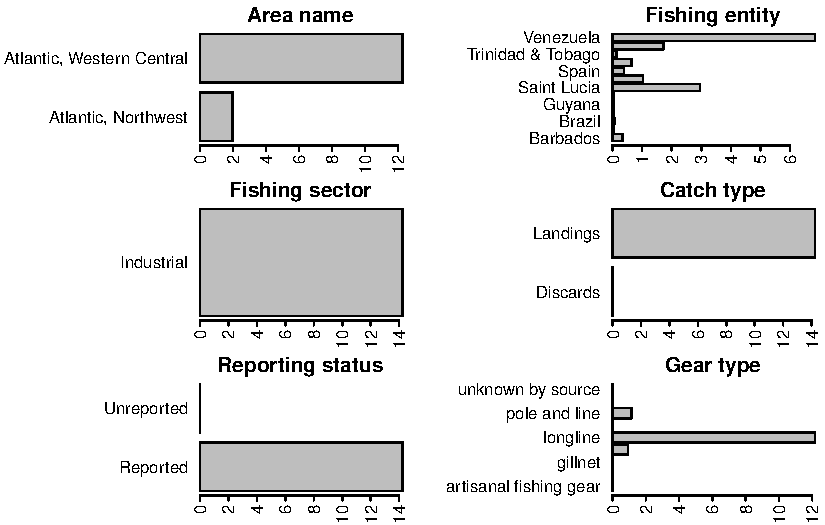
\includegraphics{SAU2_files/figure-pdf/unnamed-chunk-2-1.pdf}

\begin{Shaded}
\begin{Highlighting}[]
\FunctionTok{round}\NormalTok{(}\FunctionTok{tapply}\NormalTok{(hs}\SpecialCharTok{$}\NormalTok{pounds, hs}\SpecialCharTok{$}\NormalTok{catch\_type, sum, }\AttributeTok{na.rm =}\NormalTok{ T) }\SpecialCharTok{/} \FunctionTok{sum}\NormalTok{(hs}\SpecialCharTok{$}\NormalTok{pounds) }\SpecialCharTok{*} \DecValTok{100}\NormalTok{, }\DecValTok{2}\NormalTok{)   }\CommentTok{\# \textless{}\textless{} 1\% are discards}
\end{Highlighting}
\end{Shaded}

\begin{verbatim}
Discards Landings 
    0.03    99.97 
\end{verbatim}

\begin{Shaded}
\begin{Highlighting}[]
\FunctionTok{round}\NormalTok{(}\FunctionTok{tapply}\NormalTok{(hs}\SpecialCharTok{$}\NormalTok{pounds, hs}\SpecialCharTok{$}\NormalTok{reporting\_status, sum, }\AttributeTok{na.rm =}\NormalTok{ T) }\SpecialCharTok{/} \FunctionTok{sum}\NormalTok{(hs}\SpecialCharTok{$}\NormalTok{pounds) }\SpecialCharTok{*} \DecValTok{100}\NormalTok{, }\DecValTok{2}\NormalTok{)  }\CommentTok{\# \textless{}\textless{} 1\% are unreported}
\end{Highlighting}
\end{Shaded}

\begin{verbatim}
  Reported Unreported 
     99.97       0.03 
\end{verbatim}

Note there are few (a fraction of a percent) discards and unreported
landings -- nearly all of the high seas landings appear as reported and
landed fish.

\subsection{Summarize the high seas
landings}\label{summarize-the-high-seas-landings}

We plot the annual catches by fishing entity to look at trends over
time.

\begin{Shaded}
\begin{Highlighting}[]
\NormalTok{hs}\SpecialCharTok{$}\NormalTok{fishing\_entity }\OtherTok{\textless{}{-}} \FunctionTok{as.factor}\NormalTok{(hs}\SpecialCharTok{$}\NormalTok{fishing\_entity)}
\NormalTok{hs}\SpecialCharTok{$}\NormalTok{fishing\_entity }\OtherTok{\textless{}{-}} \FunctionTok{droplevels}\NormalTok{(hs}\SpecialCharTok{$}\NormalTok{fishing\_entity)}

\FunctionTok{par}\NormalTok{(}\AttributeTok{mar =} \FunctionTok{c}\NormalTok{(}\DecValTok{5}\NormalTok{, }\DecValTok{5}\NormalTok{, }\DecValTok{3}\NormalTok{, }\DecValTok{1}\NormalTok{), }\AttributeTok{mfrow =} \FunctionTok{c}\NormalTok{(}\DecValTok{1}\NormalTok{, }\DecValTok{1}\NormalTok{))}
\NormalTok{tab }\OtherTok{\textless{}{-}} \FunctionTok{tapply}\NormalTok{(hs}\SpecialCharTok{$}\NormalTok{pounds, }\FunctionTok{list}\NormalTok{(hs}\SpecialCharTok{$}\NormalTok{year, hs}\SpecialCharTok{$}\NormalTok{fishing\_entity), sum, }\AttributeTok{na.rm =}\NormalTok{ T)}
\FunctionTok{matplot}\NormalTok{(}\FunctionTok{as.numeric}\NormalTok{(}\FunctionTok{rownames}\NormalTok{(tab)), tab}\SpecialCharTok{/}\DecValTok{10}\SpecialCharTok{\^{}}\DecValTok{6}\NormalTok{, }\AttributeTok{type =} \StringTok{"l"}\NormalTok{, }\AttributeTok{col =} \FunctionTok{glasbey}\NormalTok{(}\FunctionTok{ncol}\NormalTok{(tab)), }\AttributeTok{lty =} \DecValTok{1}\NormalTok{, }\AttributeTok{lwd =} \DecValTok{2}\NormalTok{, }\AttributeTok{xlab =} \StringTok{"year"}\NormalTok{, }\AttributeTok{ylab =} \StringTok{"total catch (millions of pounds)"}\NormalTok{, }
        \AttributeTok{main =} \StringTok{"High seas Western Central Atlantic dolphin catch"}\NormalTok{)}
\FunctionTok{legend}\NormalTok{(}\StringTok{"topleft"}\NormalTok{, }\FunctionTok{colnames}\NormalTok{(tab), }\AttributeTok{col =} \FunctionTok{glasbey}\NormalTok{(}\FunctionTok{ncol}\NormalTok{(tab)), }\AttributeTok{lty =} \DecValTok{1}\NormalTok{, }\AttributeTok{lwd =} \DecValTok{2}\NormalTok{, }\AttributeTok{cex =} \FloatTok{0.8}\NormalTok{, }\AttributeTok{bty =} \StringTok{"n"}\NormalTok{)}
\end{Highlighting}
\end{Shaded}

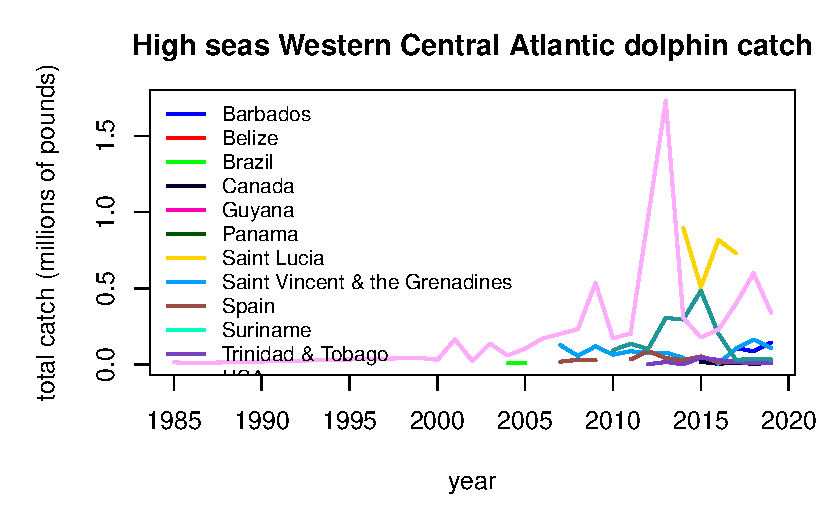
\includegraphics{SAU2_files/figure-pdf/unnamed-chunk-3-1.pdf}

Finally we output the subset of high seas dolphin catch for the two
areas. Because we have already accounted for the USA landings in our
national reporting and are aiming to only summarize international
landings here, we filter out the USA landings from the Sea Around Us
database.

\begin{Shaded}
\begin{Highlighting}[]
\NormalTok{hs }\OtherTok{\textless{}{-}}\NormalTok{ hs[}\FunctionTok{which}\NormalTok{(hs}\SpecialCharTok{$}\NormalTok{fishing\_entity }\SpecialCharTok{!=} \StringTok{"USA"}\NormalTok{), ]}

\NormalTok{hs}\SpecialCharTok{$}\NormalTok{year }\OtherTok{\textless{}{-}} \FunctionTok{factor}\NormalTok{(hs}\SpecialCharTok{$}\NormalTok{year, }\AttributeTok{levels =} \DecValTok{1950}\SpecialCharTok{:}\DecValTok{2019}\NormalTok{)}
\NormalTok{tab }\OtherTok{\textless{}{-}} \FunctionTok{tapply}\NormalTok{(hs}\SpecialCharTok{$}\NormalTok{pounds, }\FunctionTok{list}\NormalTok{(hs}\SpecialCharTok{$}\NormalTok{year, hs}\SpecialCharTok{$}\NormalTok{area\_name), sum, }\AttributeTok{na.rm =}\NormalTok{ T)}
\NormalTok{tab[}\FunctionTok{is.na}\NormalTok{(tab)] }\OtherTok{\textless{}{-}} \DecValTok{0}
\FunctionTok{tail}\NormalTok{(tab, }\DecValTok{40}\NormalTok{)}
\end{Highlighting}
\end{Shaded}

\begin{verbatim}
     Atlantic, Northwest Atlantic, Western Central
1980               0.000                     0.000
1981               0.000                     0.000
1982               0.000                     0.000
1983               0.000                     0.000
1984               0.000                     0.000
1985               0.000                 14037.129
1986               0.000                  8748.399
1987               0.000                     0.000
1988               0.000                     0.000
1989               0.000                     0.000
1990               0.000                     0.000
1991               0.000                     0.000
1992               0.000                     0.000
1993               0.000                     0.000
1994               0.000                     0.000
1995               0.000                     0.000
1996               0.000                     0.000
1997               0.000                     0.000
1998               0.000                     0.000
1999               0.000                 43168.296
2000               0.000                 30284.627
2001               0.000                164272.223
2002               0.000                 22147.477
2003               0.000                137103.181
2004               0.000                 66058.258
2005               0.000                115171.863
2006               0.000                170522.101
2007           14687.527                330838.620
2008           28552.636                340863.719
2009           18719.121                662720.661
2010            4510.085                232093.837
2011           21589.424                300498.224
2012           72398.812               1059210.392
2013           34741.604               2471791.396
2014           27922.953               1247462.983
2015           90313.638                710059.125
2016           15319.433               1094893.891
2017           34806.933               1374259.739
2018           29328.358                885814.754
2019           21870.621                632747.157
\end{verbatim}

\begin{Shaded}
\begin{Highlighting}[]
\CommentTok{\# write summary to merge with EEZ data }
\FunctionTok{write.csv}\NormalTok{(tab, }\AttributeTok{file =} \StringTok{"data/SAU/high\_seas\_by\_year.csv"}\NormalTok{)}
\end{Highlighting}
\end{Shaded}

\subsection{Distribute the high seas landings across quarters of the
year}\label{distribute-the-high-seas-landings-across-quarters-of-the-year}

The international landings are only reported as annual catches and do
not have any month or season associated with them. However, the MSE
operating model requires seasonal catches. The majority of the
international landings are caught by longline, so we will assume that
the fleet distribution of the U.S. pelagic longline is representative of
the seasonality of the international high seas fleets. Now we parse the
annual catches according to the seasonality of the U.S. fleet.

At the time of analysis, the SAU database only contained catches to
2019, so we interpolated the 2019 values to cover years 2020 - 2022.

\begin{Shaded}
\begin{Highlighting}[]
\CommentTok{\# read in the percentage of the catch by area and year{-}quarter combinations from the U.S. PLL}
\FunctionTok{load}\NormalTok{(}\StringTok{"data/per\_PLLcatch\_by\_area\_yearquarter.RData"}\NormalTok{)  }

\NormalTok{percatch[, , }\DecValTok{7}\NormalTok{] }\CommentTok{\# these are the percentages for the NED (Atlantic Northwest)}
\end{Highlighting}
\end{Shaded}

\begin{verbatim}
        1997       1998      1999        2000      2001       2002      2003
1 0.00000000 0.00000000 0.0000000 0.000000000 0.0000000 0.02866242 0.0000000
2 0.72895277 0.00000000 0.0000000 0.173761946 0.0000000 0.35668790 0.0000000
3 0.23425736 0.97257268 0.8203593 0.816681147 0.7959184 0.56050955 0.2345836
4 0.03678987 0.02742732 0.1796407 0.009556907 0.2040816 0.05414013 0.7654164
  2004 2005 2006       2007       2008        2009      2010 2011       2012
1    0  0.0    0 0.00000000 0.00000000 0.000000000 0.0000000    0 0.00000000
2    0  0.0    0 0.09846154 0.04568528 0.720183486 0.0000000    0 0.02208202
3    1  0.5    1 0.90153846 0.77157360 0.270642202 0.4885057    1 0.92744479
4    0  0.5    0 0.00000000 0.18274112 0.009174312 0.5114943    0 0.05047319
        2013      2014      2015      2016       2017       2018 2019 2020 2021
1 0.00000000 0.0000000 0.0000000 0.0000000 0.00000000 0.00000000    0    0    0
2 0.08898776 0.0000000 0.0000000 0.0000000 0.00000000 0.00000000    0    0    0
3 0.86095662 0.5979299 0.3076923 0.7073171 0.93650794 0.93650794    1    1    1
4 0.05005562 0.4020701 0.6923077 0.2926829 0.06349206 0.06349206    0    0    0
  2022
1    0
2    1
3    0
4    0
\end{verbatim}

\begin{Shaded}
\begin{Highlighting}[]
\NormalTok{tab }\OtherTok{\textless{}{-}}\NormalTok{ tab[}\FunctionTok{which}\NormalTok{(}\FunctionTok{rownames}\NormalTok{(tab) }\SpecialCharTok{\textgreater{}=} \DecValTok{1997}\NormalTok{), ]  }\CommentTok{\# PLL data are only available from 1997 on }
\CommentTok{\#tab[nrow(tab), ]}
\NormalTok{tab }\OtherTok{\textless{}{-}} \FunctionTok{rbind}\NormalTok{(tab, tab[}\FunctionTok{nrow}\NormalTok{(tab), ], tab[}\FunctionTok{nrow}\NormalTok{(tab), ], tab[}\FunctionTok{nrow}\NormalTok{(tab), ])  }\CommentTok{\# interpolate 2019 catches for 2020{-}2022}

\NormalTok{NED }\OtherTok{\textless{}{-}}\NormalTok{ percatch[, , }\DecValTok{1}\NormalTok{]   }\CommentTok{\# create matrices for final catch data}
\NormalTok{NCA }\OtherTok{\textless{}{-}}\NormalTok{ percatch[, , }\DecValTok{1}\NormalTok{]}

\ControlFlowTok{for}\NormalTok{ (i }\ControlFlowTok{in} \DecValTok{1}\SpecialCharTok{:}\FunctionTok{ncol}\NormalTok{(percatch))  \{ }
\NormalTok{  NED[, i] }\OtherTok{\textless{}{-}}\NormalTok{ percatch[, i, }\DecValTok{7}\NormalTok{] }\SpecialCharTok{*}\NormalTok{ tab[i, }\DecValTok{1}\NormalTok{]}
\NormalTok{  NCA[, i] }\OtherTok{\textless{}{-}}\NormalTok{ percatch[, i, }\DecValTok{1}\NormalTok{] }\SpecialCharTok{*}\NormalTok{ tab[i, }\DecValTok{2}\NormalTok{]}
\NormalTok{  \}}

\CommentTok{\# format for operating model}
\NormalTok{yrs }\OtherTok{\textless{}{-}} \FunctionTok{sort}\NormalTok{(}\FunctionTok{rep}\NormalTok{(}\FunctionTok{as.numeric}\NormalTok{(}\FunctionTok{colnames}\NormalTok{(NCA)), }\DecValTok{4}\NormalTok{))}
\NormalTok{qrt }\OtherTok{\textless{}{-}} \FunctionTok{rep}\NormalTok{(}\DecValTok{1}\SpecialCharTok{:}\DecValTok{4}\NormalTok{, }\FunctionTok{length}\NormalTok{(yrs)}\SpecialCharTok{/}\DecValTok{4}\NormalTok{)}
\NormalTok{flt }\OtherTok{\textless{}{-}} \FunctionTok{rep}\NormalTok{(}\StringTok{"Intl"}\NormalTok{, }\FunctionTok{length}\NormalTok{(yrs))}
\NormalTok{are }\OtherTok{\textless{}{-}} \FunctionTok{rep}\NormalTok{(}\StringTok{"NED"}\NormalTok{, }\FunctionTok{length}\NormalTok{(yrs))}
\NormalTok{fin1 }\OtherTok{\textless{}{-}} \FunctionTok{data.frame}\NormalTok{(}\FunctionTok{cbind}\NormalTok{(yrs, qrt, flt, are, }\FunctionTok{matrix}\NormalTok{(NED)))}
\NormalTok{are }\OtherTok{\textless{}{-}} \FunctionTok{rep}\NormalTok{(}\StringTok{"NCA"}\NormalTok{, }\FunctionTok{length}\NormalTok{(yrs))}
\NormalTok{fin2 }\OtherTok{\textless{}{-}} \FunctionTok{data.frame}\NormalTok{(}\FunctionTok{cbind}\NormalTok{(yrs, qrt, flt, are, }\FunctionTok{matrix}\NormalTok{(NCA)))}

\NormalTok{findat }\OtherTok{\textless{}{-}} \FunctionTok{data.frame}\NormalTok{(}\FunctionTok{rbind}\NormalTok{(fin1, fin2), }\AttributeTok{stringsAsFactors =} \ConstantTok{FALSE}\NormalTok{)}
\FunctionTok{names}\NormalTok{(findat) }\OtherTok{\textless{}{-}} \FunctionTok{c}\NormalTok{(}\StringTok{"Year"}\NormalTok{, }\StringTok{"Quarter"}\NormalTok{, }\StringTok{"Fleet"}\NormalTok{, }\StringTok{"Area"}\NormalTok{, }\StringTok{"Catch\_lbs"}\NormalTok{)}
\NormalTok{findat}\SpecialCharTok{$}\NormalTok{Catch\_lbs }\OtherTok{\textless{}{-}} \FunctionTok{as.numeric}\NormalTok{(findat}\SpecialCharTok{$}\NormalTok{Catch\_lbs)}
\FunctionTok{head}\NormalTok{(findat)}
\end{Highlighting}
\end{Shaded}

\begin{verbatim}
  Year Quarter Fleet Area Catch_lbs
1 1997       1  Intl  NED         0
2 1997       2  Intl  NED         0
3 1997       3  Intl  NED         0
4 1997       4  Intl  NED         0
5 1998       1  Intl  NED         0
6 1998       2  Intl  NED         0
\end{verbatim}

\begin{Shaded}
\begin{Highlighting}[]
\CommentTok{\#plot(findat$Catch\_lbs, type = "l")}
\CommentTok{\#plot(findat$Catch\_lbs \textasciitilde{} factor(findat$Area))}
\CommentTok{\#plot(findat$Catch\_lbs \textasciitilde{} factor(findat$Quarter))}
\CommentTok{\#plot(findat$Catch\_lbs \textasciitilde{} factor(findat$Year))}
\CommentTok{\#apply(findat, 2, table)}

\FunctionTok{write.csv}\NormalTok{(findat, }\AttributeTok{file =} \StringTok{"data/outputs/Intl\_highseas\_TomFormat.csv"}\NormalTok{)}

\NormalTok{tab }\OtherTok{\textless{}{-}} \FunctionTok{tapply}\NormalTok{(findat}\SpecialCharTok{$}\NormalTok{Catch\_lbs, }\FunctionTok{list}\NormalTok{(findat}\SpecialCharTok{$}\NormalTok{Quarter, findat}\SpecialCharTok{$}\NormalTok{Area), sum, }\AttributeTok{na.rm =}\NormalTok{ T)}
\CommentTok{\#barplot(tab, beside = T, col = rainbow(4))}

\FunctionTok{matplot}\NormalTok{(yrs }\SpecialCharTok{+}\NormalTok{ qrt}\SpecialCharTok{/}\DecValTok{4}\NormalTok{, }\FunctionTok{cbind}\NormalTok{(}\FunctionTok{as.numeric}\NormalTok{(fin1}\SpecialCharTok{$}\NormalTok{V5), }\FunctionTok{as.numeric}\NormalTok{(fin2}\SpecialCharTok{$}\NormalTok{V5))}\SpecialCharTok{/}\DecValTok{10}\SpecialCharTok{\^{}}\DecValTok{6}\NormalTok{, }\AttributeTok{lty =} \DecValTok{1}\NormalTok{, }\AttributeTok{lwd =} \DecValTok{2}\NormalTok{, }
        \AttributeTok{col =} \DecValTok{2}\SpecialCharTok{:}\DecValTok{3}\NormalTok{, }\AttributeTok{type =} \StringTok{"l"}\NormalTok{, }\AttributeTok{main =} \StringTok{"International high seas catches by quarter"}\NormalTok{, }
        \AttributeTok{xlab =} \StringTok{""}\NormalTok{, }\AttributeTok{ylab =} \StringTok{"total catch (millions of pounds)"}\NormalTok{)}
\FunctionTok{legend}\NormalTok{(}\StringTok{"topleft"}\NormalTok{, }\FunctionTok{c}\NormalTok{(}\StringTok{"NED"}\NormalTok{, }\StringTok{"NCA"}\NormalTok{), }\AttributeTok{lwd =} \DecValTok{2}\NormalTok{, }\AttributeTok{col =} \DecValTok{2}\SpecialCharTok{:}\DecValTok{3}\NormalTok{, }\AttributeTok{bty =} \StringTok{"n"}\NormalTok{)}
\end{Highlighting}
\end{Shaded}

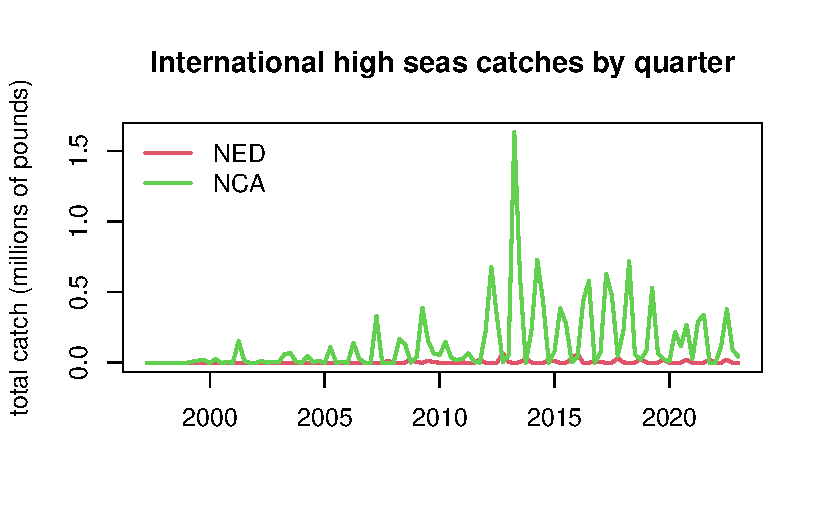
\includegraphics{SAU2_files/figure-pdf/unnamed-chunk-5-1.pdf}

\subsection{Read in the landings within excluzive economic zones
(EEZs)}\label{read-in-the-landings-within-excluzive-economic-zones-eezs}

Now we read in the landings reported by each country or jurisdiction's
respective EEZ. Because we have extracted dolphin landings for EEZs
worldwide, we need to separate out the landings for the Atlantic Ocean
basin.

\begin{Shaded}
\begin{Highlighting}[]
\FunctionTok{rm}\NormalTok{(}\AttributeTok{list =} \FunctionTok{ls}\NormalTok{())}
\NormalTok{d }\OtherTok{\textless{}{-}} \FunctionTok{read.csv}\NormalTok{(}\StringTok{"data/SAU/SAU Taxa 600006 v50{-}1.csv"}\NormalTok{, }\AttributeTok{header =}\NormalTok{ T, }\AttributeTok{sep =} \StringTok{","}\NormalTok{)  }\CommentTok{\# v. 50.1 {-} June 2024}
\FunctionTok{head}\NormalTok{(d)}
\end{Highlighting}
\end{Shaded}

\begin{verbatim}
     area_name area_type year     scientific_name        common_name
1    Australia       eez 1950 Coryphaena hippurus Common dolphinfish
2    Australia       eez 1950 Coryphaena hippurus Common dolphinfish
3    Australia       eez 1950 Coryphaena hippurus Common dolphinfish
4      Bahamas       eez 1950 Coryphaena hippurus Common dolphinfish
5     Barbados       eez 1950 Coryphaena hippurus Common dolphinfish
6 Bermuda (UK)       eez 1950 Coryphaena hippurus Common dolphinfish
          functional_group commercial_group fishing_entity fishing_sector
1 Large pelagics (>=90 cm)      Perch-likes      Australia     Industrial
2 Large pelagics (>=90 cm)      Perch-likes      Australia     Industrial
3 Large pelagics (>=90 cm)      Perch-likes      Australia     Industrial
4 Large pelagics (>=90 cm)      Perch-likes        Bahamas   Recreational
5 Large pelagics (>=90 cm)      Perch-likes       Barbados   Recreational
6 Large pelagics (>=90 cm)      Perch-likes   Bermuda (UK)      Artisanal
  catch_type reporting_status                 gear_type
1   Landings         Reported                  longline
2   Landings         Reported                  longline
3   Landings         Reported                  longline
4   Landings       Unreported recreational fishing gear
5   Landings       Unreported recreational fishing gear
6   Landings         Reported         small scale lines
              end_use_type       tonnes landed_value
1    Fishmeal and fish oil  0.003373202 3.438170e-05
2 Direct human consumption  6.739657104 1.040254e+04
3                    Other  0.003373202 3.438170e-05
4 Direct human consumption 48.665105143 8.262728e+00
5 Direct human consumption  0.009158559 4.846886e-04
6 Direct human consumption  1.511085514 3.199403e+03
\end{verbatim}

\begin{Shaded}
\begin{Highlighting}[]
\CommentTok{\#dim(d)}
\CommentTok{\#apply(d[1:13], 2, table)}

\CommentTok{\# convert tonnes to pounds }
\NormalTok{d}\SpecialCharTok{$}\NormalTok{lbs }\OtherTok{\textless{}{-}}\NormalTok{ d}\SpecialCharTok{$}\NormalTok{tonnes }\SpecialCharTok{*} \DecValTok{1000} \SpecialCharTok{*} \FloatTok{2.20462}
\end{Highlighting}
\end{Shaded}

We look at the characteristics of the landings within EEZs. These are
largely industrial and artisanal in nature. Landings are the majority of
the catch but discards are also present. There are more unreported
landings than reported landings and a variety of gear types are used.

\begin{Shaded}
\begin{Highlighting}[]
\CommentTok{\# look at characteristics of data }
\FunctionTok{par}\NormalTok{(}\AttributeTok{mfrow =} \FunctionTok{c}\NormalTok{(}\DecValTok{2}\NormalTok{, }\DecValTok{2}\NormalTok{), }\AttributeTok{mar =} \FunctionTok{c}\NormalTok{(}\DecValTok{12}\NormalTok{, }\DecValTok{7}\NormalTok{, }\DecValTok{3}\NormalTok{, }\DecValTok{1}\NormalTok{), }\AttributeTok{mex =} \FloatTok{0.5}\NormalTok{, }\AttributeTok{mgp =} \FunctionTok{c}\NormalTok{(}\DecValTok{5}\NormalTok{, }\DecValTok{1}\NormalTok{, }\DecValTok{0}\NormalTok{))}
\FunctionTok{barplot}\NormalTok{(}\FunctionTok{tapply}\NormalTok{(d}\SpecialCharTok{$}\NormalTok{lbs, d}\SpecialCharTok{$}\NormalTok{fishing\_sector, sum, }\AttributeTok{na.rm =}\NormalTok{ T)}\SpecialCharTok{/}\DecValTok{10}\SpecialCharTok{\^{}}\DecValTok{6}\NormalTok{, }\AttributeTok{las =} \DecValTok{2}\NormalTok{, }\AttributeTok{ylab =} \StringTok{"millions of pounds"}\NormalTok{, }\AttributeTok{main =} \StringTok{"Fishing sector"}\NormalTok{)}
\FunctionTok{barplot}\NormalTok{(}\FunctionTok{tapply}\NormalTok{(d}\SpecialCharTok{$}\NormalTok{lbs, d}\SpecialCharTok{$}\NormalTok{catch\_type, sum, }\AttributeTok{na.rm =}\NormalTok{ T)}\SpecialCharTok{/}\DecValTok{10}\SpecialCharTok{\^{}}\DecValTok{6}\NormalTok{, }\AttributeTok{las =} \DecValTok{2}\NormalTok{, }\AttributeTok{ylab =} \StringTok{"millions of pounds"}\NormalTok{, }\AttributeTok{main =} \StringTok{"Catch type"}\NormalTok{)}
\FunctionTok{barplot}\NormalTok{(}\FunctionTok{tapply}\NormalTok{(d}\SpecialCharTok{$}\NormalTok{lbs, d}\SpecialCharTok{$}\NormalTok{reporting\_status, sum, }\AttributeTok{na.rm =}\NormalTok{ T)}\SpecialCharTok{/}\DecValTok{10}\SpecialCharTok{\^{}}\DecValTok{6}\NormalTok{, }\AttributeTok{las =} \DecValTok{2}\NormalTok{, }\AttributeTok{ylab =} \StringTok{"millions of pounds"}\NormalTok{, }\AttributeTok{main =} \StringTok{"Reporting status"}\NormalTok{)}
\FunctionTok{barplot}\NormalTok{(}\FunctionTok{tapply}\NormalTok{(d}\SpecialCharTok{$}\NormalTok{lbs, d}\SpecialCharTok{$}\NormalTok{gear\_type, sum, }\AttributeTok{na.rm =}\NormalTok{ T)}\SpecialCharTok{/}\DecValTok{10}\SpecialCharTok{\^{}}\DecValTok{6}\NormalTok{, }\AttributeTok{las =} \DecValTok{2}\NormalTok{, }\AttributeTok{ylab =} \StringTok{"millions of pounds"}\NormalTok{, }\AttributeTok{main =} \StringTok{"Gear type"}\NormalTok{)}
\end{Highlighting}
\end{Shaded}

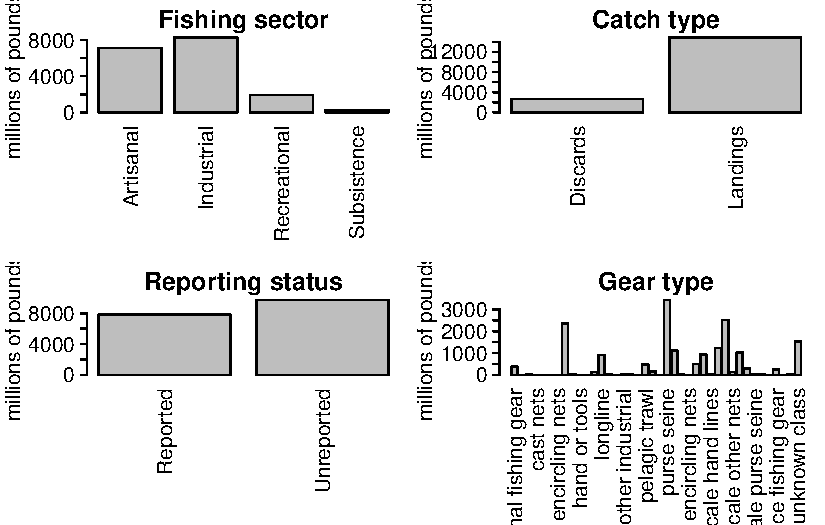
\includegraphics{SAU2_files/figure-pdf/unnamed-chunk-7-1.pdf}

\subsection{Separating the EEZs by
area}\label{separating-the-eezs-by-area}

Now we have to manually assign the different EEZs to respective areas.
We separate the geographical areas within the Atlantic Ocean (North and
South) and lump all other EEZs into ``other oceans.'' This latter
category is largely the Pacific Ocean and to a lesser extent the Indian
Ocean. We remove the high seas catch from this database as it is not
ocean-specific and we have extracted the ocean-specific high seas catch
previously.

\begin{Shaded}
\begin{Highlighting}[]
\CommentTok{\# remove the high seas catch from this database}
\NormalTok{d }\OtherTok{\textless{}{-}}\NormalTok{ d[}\FunctionTok{which}\NormalTok{(d}\SpecialCharTok{$}\NormalTok{area\_type }\SpecialCharTok{!=} \StringTok{"high\_seas"}\NormalTok{), ]   }
\NormalTok{d}\SpecialCharTok{$}\NormalTok{fishing\_entity }\OtherTok{\textless{}{-}} \FunctionTok{as.factor}\NormalTok{(d}\SpecialCharTok{$}\NormalTok{fishing\_entity)}
\NormalTok{d}\SpecialCharTok{$}\NormalTok{fishing\_entity }\OtherTok{\textless{}{-}} \FunctionTok{droplevels}\NormalTok{(d}\SpecialCharTok{$}\NormalTok{fishing\_entity)}
\FunctionTok{table}\NormalTok{(d}\SpecialCharTok{$}\NormalTok{area\_type)  }\CommentTok{\# this should be all "eez"}
\end{Highlighting}
\end{Shaded}

\begin{verbatim}

  eez 
63056 
\end{verbatim}

\begin{Shaded}
\begin{Highlighting}[]
\CommentTok{\# Western Central Atlantic EEZs}
\NormalTok{WCA }\OtherTok{\textless{}{-}} \FunctionTok{c}\NormalTok{(}\StringTok{"Bahamas"}\NormalTok{, }\StringTok{"Barbados"}\NormalTok{, }\StringTok{"Cayman Isl. (UK)"}\NormalTok{, }\StringTok{"Dominica"}\NormalTok{, }\StringTok{"Dominican Republic"}\NormalTok{, }\StringTok{"Grenada"}\NormalTok{, }
         \StringTok{"Aruba (Netherlands)"}\NormalTok{, }\StringTok{"Haiti"}\NormalTok{, }\StringTok{"Guadeloupe  (France)"}\NormalTok{, }\StringTok{"Jamaica"}\NormalTok{, }\StringTok{"Martinique (France)"}\NormalTok{,}
         \StringTok{"Montserrat (UK)"}\NormalTok{, }\StringTok{"Nicaragua (Caribbean)"}\NormalTok{, }\StringTok{"Puerto Rico (USA)"}\NormalTok{, }\StringTok{"Saint Kitts \& Nevis"}\NormalTok{, }
         \StringTok{"Saint Lucia"}\NormalTok{, }\StringTok{"Saint Vincent \& the Grenadines"}\NormalTok{, }\StringTok{"Trinidad \& Tobago"}\NormalTok{, }\StringTok{"US Virgin Isl."}\NormalTok{, }
         \StringTok{"St Barthelemy (France)"}\NormalTok{, }\StringTok{"St Martin (France)"}\NormalTok{, }\StringTok{"Curaçao (Netherlands)"}\NormalTok{, }\StringTok{"Bonaire (Netherlands)"}\NormalTok{,}
         \StringTok{"Saba and Sint Eustatius (Netherlands)"}\NormalTok{, }\StringTok{"Sint Maarten (Netherlands)"}\NormalTok{, }\StringTok{"Honduras (Caribbean)"}\NormalTok{,}
         \StringTok{"Colombia (Caribbean)"}\NormalTok{, }\StringTok{"Mexico (Atlantic)"}\NormalTok{, }\StringTok{"Turks \& Caicos Isl. (UK)"}\NormalTok{, }\StringTok{"Guyana"}\NormalTok{, }\StringTok{"Venezuela"}\NormalTok{,}
         \StringTok{"Antigua \& Barbuda"}\NormalTok{, }\StringTok{"Belize"}\NormalTok{, }\StringTok{"British Virgin Isl. (UK)"}\NormalTok{, }\StringTok{"French Guiana"}\NormalTok{, }\StringTok{"Cuba"}\NormalTok{, }
         \StringTok{"Anguilla (UK)"}\NormalTok{, }\StringTok{"Suriname"}\NormalTok{, }\StringTok{"Costa Rica (Caribbean)"}\NormalTok{, }\StringTok{"Guatemala (Caribbean)"}\NormalTok{, }
         \StringTok{"Panama (Caribbean)"}\NormalTok{, }\StringTok{"Bermuda (UK)"}\NormalTok{, }\StringTok{"Curaçao (Netherlands)"}\NormalTok{) }
           
\CommentTok{\# Brazil}
\NormalTok{Bra }\OtherTok{\textless{}{-}} \FunctionTok{c}\NormalTok{(}\StringTok{"Brazil (mainland)"}\NormalTok{, }\StringTok{"Fernando de Noronha (Brazil)"}\NormalTok{, }
         \StringTok{"St Paul and St. Peter Archipelago (Brazil)"}\NormalTok{)}

\CommentTok{\# Canada}
\NormalTok{Can }\OtherTok{\textless{}{-}}  \FunctionTok{c}\NormalTok{(}\StringTok{"Canada (East Coast)"}\NormalTok{, }\StringTok{"Saint Pierre \& Miquelon (France)"}\NormalTok{)}

\CommentTok{\# United States}
\NormalTok{USA }\OtherTok{\textless{}{-}}  \FunctionTok{c}\NormalTok{(}\StringTok{"USA (East Coast)"}\NormalTok{, }\StringTok{"USA (Gulf of Mexico)"}\NormalTok{)}
           
\CommentTok{\# Northeast Atlantic EEZs}
\NormalTok{NEA }\OtherTok{\textless{}{-}} \FunctionTok{c}\NormalTok{(}\StringTok{"Canary Isl. (Spain)"}\NormalTok{, }\StringTok{"Spain (mainland; Med and Gulf of Cadiz)"}\NormalTok{, }\StringTok{"Spain (Northwest)"}\NormalTok{, }
         \StringTok{"Spain (mainland, Med and Gulf of Cadiz)"}\NormalTok{, }
         \StringTok{"France (Atlantic Coast)"}\NormalTok{, }\StringTok{"Portugal (mainland)"}\NormalTok{, }\StringTok{"Azores Isl. (Portugal)"}\NormalTok{)}
        
\CommentTok{\# Eastern Central Atlantic EEZs}
\NormalTok{ECA }\OtherTok{\textless{}{-}} \FunctionTok{c}\NormalTok{(}\StringTok{"Madeira Isl. (Portugal)"}\NormalTok{, }\StringTok{"Cape Verde"}\NormalTok{, }\StringTok{"Equatorial Guinea"}\NormalTok{, }\StringTok{"Benin"}\NormalTok{, }
          \StringTok{"Sao Tome \& Principe "}\NormalTok{, }\StringTok{"Sao Tome \& Principe"}\NormalTok{, }\StringTok{"Morocco (Central)"}\NormalTok{, }\StringTok{"Ghana"}\NormalTok{, }
          \StringTok{"Côte d\textquotesingle{}Ivoire"}\NormalTok{, }\StringTok{"Côte d\textquotesingle{}Ivoire"}\NormalTok{, }\StringTok{"Guinea"}\NormalTok{, }\StringTok{"Liberia"}\NormalTok{, }\StringTok{"Sierra Leone"}\NormalTok{, }\StringTok{"Nigeria"}\NormalTok{, }\StringTok{"Togo"}\NormalTok{, }
          \StringTok{"Guinea{-}Bissau"}\NormalTok{, }\StringTok{"Senegal"}\NormalTok{, }\StringTok{"Cameroon"}\NormalTok{, }\StringTok{"Gambia"}\NormalTok{, }\StringTok{"Mauritania"}\NormalTok{, }\StringTok{"Morocco (South)"}\NormalTok{, }
          \StringTok{"Gabon"}\NormalTok{, }\StringTok{"Congo; R. of"}\NormalTok{, }\StringTok{"Congo, R. of"}\NormalTok{, }\StringTok{"Congo (ex{-}Zaire)"}\NormalTok{)}

\CommentTok{\# Southeastern Atlantic EEZs}
\NormalTok{SEA }\OtherTok{\textless{}{-}} \FunctionTok{c}\NormalTok{(}\StringTok{"Angola"}\NormalTok{, }\StringTok{"Namibia"}\NormalTok{, }\StringTok{"South Africa (Atlantic and Cape)"}\NormalTok{,  }
           \StringTok{"Ascension Isl. (UK)"}\NormalTok{, }\StringTok{"Saint Helena (UK)"}\NormalTok{, }\StringTok{"Tristan da Cunha Isl. (UK)"}\NormalTok{)}

\CommentTok{\# Southwest Atlantic EEZs}
\NormalTok{SWA }\OtherTok{\textless{}{-}} \FunctionTok{c}\NormalTok{(}\StringTok{"Trindade \& Martim Vaz Isl. (Brazil)"}\NormalTok{, }\StringTok{"Uruguay"}\NormalTok{)}

\CommentTok{\# Mediterranean EEZs}
\NormalTok{Med }\OtherTok{\textless{}{-}} \FunctionTok{c}\NormalTok{(}\StringTok{"Italy (mainland)"}\NormalTok{, }\StringTok{"Libya"}\NormalTok{, }\StringTok{"Malta"}\NormalTok{, }\StringTok{"Syria"}\NormalTok{, }\StringTok{"Sicily (Italy)"}\NormalTok{,}\StringTok{"Sardinia (Italy)"}\NormalTok{, }
         \StringTok{"Balearic Islands (Spain)"}\NormalTok{, }\StringTok{"Cyprus (North)"}\NormalTok{, }\StringTok{"Cyprus (South)"}\NormalTok{, }
         \StringTok{"Gaza Strip"}\NormalTok{, }\StringTok{"Greece (without Crete)"}\NormalTok{, }\StringTok{"Crete (Greece)"}\NormalTok{, }\StringTok{"Lebanon"}\NormalTok{, }
         \StringTok{"Turkey (Mediterranean Sea)"}\NormalTok{, }\StringTok{"Egypt (Mediterranean)"}\NormalTok{, }\StringTok{"Israel (Mediterranean)"}\NormalTok{, }\StringTok{"Tunisia"}\NormalTok{, }
         \StringTok{"Algeria"}\NormalTok{, }\StringTok{"Albania"}\NormalTok{, }\StringTok{"Croatia"}\NormalTok{, }\StringTok{"Montenegro"}\NormalTok{, }\StringTok{"Morocco (Mediterranean)"}\NormalTok{, }
         \StringTok{"France (Mediterranean)"}\NormalTok{, }\StringTok{"Corsica (France)"}\NormalTok{)}

\CommentTok{\# add variable to specify region}
\NormalTok{d}\SpecialCharTok{$}\NormalTok{reg }\OtherTok{\textless{}{-}} \StringTok{"other oceans"}
\NormalTok{d}\SpecialCharTok{$}\NormalTok{reg[}\FunctionTok{which}\NormalTok{(d}\SpecialCharTok{$}\NormalTok{area\_name }\SpecialCharTok{\%in\%}\NormalTok{ WCA)] }\OtherTok{\textless{}{-}} \StringTok{"Western Central Atlantic EEZs"}
\NormalTok{d}\SpecialCharTok{$}\NormalTok{reg[}\FunctionTok{which}\NormalTok{(d}\SpecialCharTok{$}\NormalTok{area\_name }\SpecialCharTok{\%in\%}\NormalTok{ Bra)] }\OtherTok{\textless{}{-}} \StringTok{"Brazil EEZ"}
\NormalTok{d}\SpecialCharTok{$}\NormalTok{reg[}\FunctionTok{which}\NormalTok{(d}\SpecialCharTok{$}\NormalTok{area\_name }\SpecialCharTok{\%in\%}\NormalTok{ Can)] }\OtherTok{\textless{}{-}} \StringTok{"Canadian EEZ"}
\NormalTok{d}\SpecialCharTok{$}\NormalTok{reg[}\FunctionTok{which}\NormalTok{(d}\SpecialCharTok{$}\NormalTok{area\_name }\SpecialCharTok{\%in\%}\NormalTok{ USA)] }\OtherTok{\textless{}{-}} \StringTok{"United States EEZ"}
\NormalTok{d}\SpecialCharTok{$}\NormalTok{reg[}\FunctionTok{which}\NormalTok{(d}\SpecialCharTok{$}\NormalTok{area\_name }\SpecialCharTok{\%in\%}\NormalTok{ NEA)] }\OtherTok{\textless{}{-}} \StringTok{"Northeast Atlantic EEZs"}
\NormalTok{d}\SpecialCharTok{$}\NormalTok{reg[}\FunctionTok{which}\NormalTok{(d}\SpecialCharTok{$}\NormalTok{area\_name }\SpecialCharTok{\%in\%}\NormalTok{ ECA)] }\OtherTok{\textless{}{-}} \StringTok{"Eastern Central Atlantic EEZs"}
\NormalTok{d}\SpecialCharTok{$}\NormalTok{reg[}\FunctionTok{which}\NormalTok{(d}\SpecialCharTok{$}\NormalTok{area\_name }\SpecialCharTok{\%in\%}\NormalTok{ SEA)] }\OtherTok{\textless{}{-}} \StringTok{"Southeast Atlantic EEZs"}
\NormalTok{d}\SpecialCharTok{$}\NormalTok{reg[}\FunctionTok{which}\NormalTok{(d}\SpecialCharTok{$}\NormalTok{area\_name }\SpecialCharTok{\%in\%}\NormalTok{ SWA)] }\OtherTok{\textless{}{-}} \StringTok{"Southwest Atlantic EEZs"}
\NormalTok{d}\SpecialCharTok{$}\NormalTok{reg[}\FunctionTok{which}\NormalTok{(d}\SpecialCharTok{$}\NormalTok{area\_name }\SpecialCharTok{\%in\%}\NormalTok{ Med)] }\OtherTok{\textless{}{-}} \StringTok{"Mediterranean Sea EEZs"}
\end{Highlighting}
\end{Shaded}

Now we will check that we have classified the regions correctly.

\begin{Shaded}
\begin{Highlighting}[]
\CommentTok{\# check region designation }
\NormalTok{othlis }\OtherTok{\textless{}{-}} \FunctionTok{unique}\NormalTok{(d}\SpecialCharTok{$}\NormalTok{area\_name[}\FunctionTok{which}\NormalTok{(d}\SpecialCharTok{$}\NormalTok{reg }\SpecialCharTok{==} \StringTok{"other oceans"}\NormalTok{)])}
\FunctionTok{print}\NormalTok{(}\StringTok{"EEZs of all other oceans: "}\NormalTok{)}
\end{Highlighting}
\end{Shaded}

\begin{verbatim}
[1] "EEZs of all other oceans: "
\end{verbatim}

\begin{Shaded}
\begin{Highlighting}[]
\NormalTok{othlis}
\end{Highlighting}
\end{Shaded}

\begin{verbatim}
  [1] "Australia"                          "China"                             
  [3] "Taiwan"                             "Mayotte (France)"                  
  [5] "French Polynesia"                   "Hong Kong (China)"                 
  [7] "Andaman & Nicobar Isl. (India)"     "Indonesia (Eastern)"               
  [9] "Japan (main islands)"               "Japan (Daito Islands)"             
 [11] "Korea (South)"                      "Hawaii Northwest Islands (USA)"    
 [13] "Nauru"                              "Niue (New Zealand)"                
 [15] "Northern Marianas (USA)"            "Micronesia (Federated States of)"  
 [17] "Marshall Isl."                      "Palau"                             
 [19] "Pakistan"                           "Papua New Guinea"                  
 [21] "Philippines"                        "Seychelles"                        
 [23] "Viet Nam"                           "Tokelau (New Zealand)"             
 [25] "Tonga"                              "Hawaii Main Islands (USA)"         
 [27] "USA (West Coast)"                   "Wake Isl. (USA)"                   
 [29] "Wallis & Futuna Isl. (France)"      "Samoa"                             
 [31] "Guatemala (Pacific)"                "Kiribati (Gilbert Islands)"        
 [33] "Mexico (Pacific)"                   "Japan (Ogasawara Islands)"         
 [35] "Korea (North, Yellow Sea)"          "Korea (North, Sea of Japan)"       
 [37] "Mauritius"                          "Solomon Isl."                      
 [39] "Christmas Isl. (Australia)"         "Johnston Atoll (USA)"              
 [41] "Timor Leste"                        "Palmyra Atoll & Kingman Reef (USA)"
 [43] "Jarvis Isl. (USA)"                  "Howland & Baker Isl. (USA)"        
 [45] "Indonesia (Central)"                "Indonesia (Indian Ocean)"          
 [47] "Kiribati (Line Islands)"            "Kiribati (Phoenix Islands)"        
 [49] "New Caledonia (France)"             "Vanuatu"                           
 [51] "Lord Howe Isl. (Australia)"         "Myanmar"                           
 [53] "Ecuador (mainland)"                 "El Salvador"                       
 [55] "Fiji"                               "Malaysia (Peninsula West)"         
 [57] "Norfolk Isl. (Australia)"           "Peru"                              
 [59] "Pitcairn (UK)"                      "Colombia (Pacific)"                
 [61] "Costa Rica (Pacific)"               "Nicaragua (Pacific)"               
 [63] "Panama (Pacific)"                   "Thailand (Andaman Sea)"            
 [65] "Thailand (Gulf of Thailand)"        "Cook Islands"                      
 [67] "Kermadec Isl. (New Zealand)"        "Tuvalu"                            
 [69] "Honduras (Pacific)"                 "American Samoa"                    
 [71] "Galapagos Isl. (Ecuador)"           "New Zealand"                       
 [73] "Brunei Darussalam"                  "Malaysia (Sabah)"                  
 [75] "Malaysia (Sarawak)"                 "Guam (USA)"                        
 [77] "Clipperton Isl. (France)"           "South Africa (Indian Ocean Coast)" 
 [79] "Singapore"                          "Easter Isl. (Chile)"               
 [81] "Madagascar"                         "Réunion (France)"                  
 [83] "Chagos Archipelago (UK)"            "Comoros Isl."                      
 [85] "Mozambique Channel Isl. (France)"   "Kenya"                             
 [87] "Mozambique"                         "Somalia"                           
 [89] "Tanzania"                           "Glorieuse Islands (France)"        
 [91] "Yemen (Socotra)"                    "Oman"                              
 [93] "St Paul & Amsterdam Isl. (France)"  "Iran (Sea of Oman)"                
 [95] "Desventuradas Isl. (Chile)"         "India (mainland)"                  
 [97] "Maldives"                           "Tromelin Isl. (France)"            
 [99] "Cambodia"                           "Sri Lanka"                         
[101] "Malaysia (Peninsula East)"          "Bangladesh"                        
\end{verbatim}

\begin{Shaded}
\begin{Highlighting}[]
\FunctionTok{print}\NormalTok{(}\StringTok{"U.S. EEZs outside the Atlantic Ocean: "}\NormalTok{)}
\end{Highlighting}
\end{Shaded}

\begin{verbatim}
[1] "U.S. EEZs outside the Atlantic Ocean: "
\end{verbatim}

\begin{Shaded}
\begin{Highlighting}[]
\NormalTok{othlis[}\FunctionTok{grep}\NormalTok{(}\StringTok{"USA"}\NormalTok{, othlis)]}
\end{Highlighting}
\end{Shaded}

\begin{verbatim}
 [1] "Hawaii Northwest Islands (USA)"     "Northern Marianas (USA)"           
 [3] "Hawaii Main Islands (USA)"          "USA (West Coast)"                  
 [5] "Wake Isl. (USA)"                    "Johnston Atoll (USA)"              
 [7] "Palmyra Atoll & Kingman Reef (USA)" "Jarvis Isl. (USA)"                 
 [9] "Howland & Baker Isl. (USA)"         "Guam (USA)"                        
\end{verbatim}

\begin{Shaded}
\begin{Highlighting}[]
\FunctionTok{print}\NormalTok{(}\StringTok{"French EEZs outside the Atlantic Ocean: "}\NormalTok{)}
\end{Highlighting}
\end{Shaded}

\begin{verbatim}
[1] "French EEZs outside the Atlantic Ocean: "
\end{verbatim}

\begin{Shaded}
\begin{Highlighting}[]
\NormalTok{othlis[}\FunctionTok{grep}\NormalTok{(}\StringTok{"France"}\NormalTok{, othlis)]}
\end{Highlighting}
\end{Shaded}

\begin{verbatim}
[1] "Mayotte (France)"                  "Wallis & Futuna Isl. (France)"    
[3] "New Caledonia (France)"            "Clipperton Isl. (France)"         
[5] "Réunion (France)"                  "Mozambique Channel Isl. (France)" 
[7] "Glorieuse Islands (France)"        "St Paul & Amsterdam Isl. (France)"
[9] "Tromelin Isl. (France)"           
\end{verbatim}

\begin{Shaded}
\begin{Highlighting}[]
\FunctionTok{unique}\NormalTok{(d}\SpecialCharTok{$}\NormalTok{area\_name[}\FunctionTok{which}\NormalTok{(d}\SpecialCharTok{$}\NormalTok{reg }\SpecialCharTok{==} \StringTok{"Western Central Atlantic EEZs"}\NormalTok{)])   }\CommentTok{\# Western Central EEZs:}
\end{Highlighting}
\end{Shaded}

\begin{verbatim}
 [1] "Bahamas"                              
 [2] "Barbados"                             
 [3] "Bermuda (UK)"                         
 [4] "Cayman Isl. (UK)"                     
 [5] "Dominica"                             
 [6] "Dominican Republic"                   
 [7] "Grenada"                              
 [8] "Guadeloupe  (France)"                 
 [9] "Haiti"                                
[10] "Jamaica"                              
[11] "Martinique (France)"                  
[12] "Montserrat (UK)"                      
[13] "Puerto Rico (USA)"                    
[14] "Saint Kitts & Nevis"                  
[15] "Saint Lucia"                          
[16] "Saint Vincent & the Grenadines"       
[17] "Trinidad & Tobago"                    
[18] "US Virgin Isl."                       
[19] "St Barthelemy (France)"               
[20] "St Martin (France)"                   
[21] "Curaçao (Netherlands)"                
[22] "Bonaire (Netherlands)"                
[23] "Saba and Sint Eustatius (Netherlands)"
[24] "Sint Maarten (Netherlands)"           
[25] "Honduras (Caribbean)"                 
[26] "Colombia (Caribbean)"                 
[27] "Mexico (Atlantic)"                    
[28] "Turks & Caicos Isl. (UK)"             
[29] "Costa Rica (Caribbean)"               
[30] "Panama (Caribbean)"                   
[31] "Antigua & Barbuda"                    
[32] "Belize"                               
[33] "British Virgin Isl. (UK)"             
[34] "Cuba"                                 
[35] "French Guiana"                        
[36] "Guyana"                               
[37] "Anguilla (UK)"                        
[38] "Suriname"                             
[39] "Venezuela"                            
[40] "Guatemala (Caribbean)"                
[41] "Aruba (Netherlands)"                  
[42] "Nicaragua (Caribbean)"                
\end{verbatim}

\begin{Shaded}
\begin{Highlighting}[]
\FunctionTok{unique}\NormalTok{(d}\SpecialCharTok{$}\NormalTok{area\_name[}\FunctionTok{which}\NormalTok{(d}\SpecialCharTok{$}\NormalTok{reg }\SpecialCharTok{==} \StringTok{"Brazil EEZ"}\NormalTok{)])   }\CommentTok{\# Brazil EEZs:}
\end{Highlighting}
\end{Shaded}

\begin{verbatim}
[1] "Brazil (mainland)"                         
[2] "Fernando de Noronha (Brazil)"              
[3] "St Paul and St. Peter Archipelago (Brazil)"
\end{verbatim}

\begin{Shaded}
\begin{Highlighting}[]
\FunctionTok{unique}\NormalTok{(d}\SpecialCharTok{$}\NormalTok{area\_name[}\FunctionTok{which}\NormalTok{(d}\SpecialCharTok{$}\NormalTok{reg }\SpecialCharTok{==} \StringTok{"Canadian EEZ"}\NormalTok{)])   }\CommentTok{\# Canadian EEZs:}
\end{Highlighting}
\end{Shaded}

\begin{verbatim}
[1] "Canada (East Coast)"              "Saint Pierre & Miquelon (France)"
\end{verbatim}

\begin{Shaded}
\begin{Highlighting}[]
\FunctionTok{unique}\NormalTok{(d}\SpecialCharTok{$}\NormalTok{area\_name[}\FunctionTok{which}\NormalTok{(d}\SpecialCharTok{$}\NormalTok{reg }\SpecialCharTok{==} \StringTok{"United States EEZ"}\NormalTok{)])  }\CommentTok{\# United States EEZs:}
\end{Highlighting}
\end{Shaded}

\begin{verbatim}
[1] "USA (East Coast)"     "USA (Gulf of Mexico)"
\end{verbatim}

\begin{Shaded}
\begin{Highlighting}[]
\FunctionTok{unique}\NormalTok{(d}\SpecialCharTok{$}\NormalTok{area\_name[}\FunctionTok{which}\NormalTok{(d}\SpecialCharTok{$}\NormalTok{reg }\SpecialCharTok{==} \StringTok{"Northeast Atlantic EEZs"}\NormalTok{)])   }\CommentTok{\# Northeast Atlantic EEZs:}
\end{Highlighting}
\end{Shaded}

\begin{verbatim}
[1] "Azores Isl. (Portugal)"                 
[2] "Spain (mainland, Med and Gulf of Cadiz)"
[3] "Canary Isl. (Spain)"                    
[4] "Portugal (mainland)"                    
[5] "France (Atlantic Coast)"                
[6] "Spain (Northwest)"                      
\end{verbatim}

\begin{Shaded}
\begin{Highlighting}[]
\FunctionTok{unique}\NormalTok{(d}\SpecialCharTok{$}\NormalTok{area\_name[}\FunctionTok{which}\NormalTok{(d}\SpecialCharTok{$}\NormalTok{reg }\SpecialCharTok{==} \StringTok{"Eastern Central Atlantic EEZs"}\NormalTok{)])   }\CommentTok{\# Eastern Central Atlantic EEZs:}
\end{Highlighting}
\end{Shaded}

\begin{verbatim}
 [1] "Cape Verde"              "Equatorial Guinea"      
 [3] "Sao Tome & Principe"     "Madeira Isl. (Portugal)"
 [5] "Togo"                    "Ghana"                  
 [7] "Guinea"                  "Liberia"                
 [9] "Guinea-Bissau"           "Senegal"                
[11] "Sierra Leone"            "Morocco (Central)"      
[13] "Morocco (South)"         "Côte d'Ivoire"          
[15] "Gabon"                   "Benin"                  
[17] "Gambia"                  "Mauritania"             
[19] "Nigeria"                 "Cameroon"               
[21] "Congo, R. of"            "Congo (ex-Zaire)"       
\end{verbatim}

\begin{Shaded}
\begin{Highlighting}[]
\FunctionTok{unique}\NormalTok{(d}\SpecialCharTok{$}\NormalTok{area\_name[}\FunctionTok{which}\NormalTok{(d}\SpecialCharTok{$}\NormalTok{reg }\SpecialCharTok{==} \StringTok{"Southeast Atlantic EEZs"}\NormalTok{)])   }\CommentTok{\# Southeast Atlantic EEZs:}
\end{Highlighting}
\end{Shaded}

\begin{verbatim}
[1] "Ascension Isl. (UK)"              "South Africa (Atlantic and Cape)"
[3] "Saint Helena (UK)"                "Angola"                          
[5] "Namibia"                          "Tristan da Cunha Isl. (UK)"      
\end{verbatim}

\begin{Shaded}
\begin{Highlighting}[]
\FunctionTok{unique}\NormalTok{(d}\SpecialCharTok{$}\NormalTok{area\_name[}\FunctionTok{which}\NormalTok{(d}\SpecialCharTok{$}\NormalTok{reg }\SpecialCharTok{==} \StringTok{"Southwest Atlantic EEZs"}\NormalTok{)])   }\CommentTok{\# Southwest Atlantic EEZs:}
\end{Highlighting}
\end{Shaded}

\begin{verbatim}
[1] "Trindade & Martim Vaz Isl. (Brazil)" "Uruguay"                            
\end{verbatim}

\begin{Shaded}
\begin{Highlighting}[]
\FunctionTok{unique}\NormalTok{(d}\SpecialCharTok{$}\NormalTok{area\_name[}\FunctionTok{which}\NormalTok{(d}\SpecialCharTok{$}\NormalTok{reg }\SpecialCharTok{==} \StringTok{"Mediterranean Sea EEZs"}\NormalTok{)])   }\CommentTok{\# Mediterranean Sea EEZs:}
\end{Highlighting}
\end{Shaded}

\begin{verbatim}
 [1] "Italy (mainland)"         "Libya"                   
 [3] "Malta"                    "Syria"                   
 [5] "Sicily (Italy)"           "Sardinia (Italy)"        
 [7] "Balearic Islands (Spain)" "Tunisia"                 
 [9] "Algeria"                  "Morocco (Mediterranean)" 
[11] "France (Mediterranean)"   "Corsica (France)"        
[13] "Croatia"                  "Lebanon"                 
[15] "Albania"                  "Greece (without Crete)"  
[17] "Crete (Greece)"           "Cyprus (South)"          
\end{verbatim}

\subsection{Summarize catch by regional
EEZs}\label{summarize-catch-by-regional-eezs}

Now we will summarize the catch by region by grouping the catch across
the EEZs by region and plot the results. The U.S. landings should be
very close to what is reported in Section 2 because the majority of U.S.
catch is reported through the various data collection systems that are
compiled within Sea Around Us.

\begin{Shaded}
\begin{Highlighting}[]
\CommentTok{\# summarize EEZ catch by region}
\NormalTok{tab }\OtherTok{\textless{}{-}} \FunctionTok{tapply}\NormalTok{(d}\SpecialCharTok{$}\NormalTok{lbs, }\FunctionTok{list}\NormalTok{(d}\SpecialCharTok{$}\NormalTok{year, d}\SpecialCharTok{$}\NormalTok{reg), sum, }\AttributeTok{na.rm =}\NormalTok{ T)}
\CommentTok{\#head(tab)}
\NormalTok{tab2 }\OtherTok{\textless{}{-}} \FunctionTok{t}\NormalTok{(tab)}
\NormalTok{tab3 }\OtherTok{\textless{}{-}}\NormalTok{ tab2[}\FunctionTok{order}\NormalTok{(}\FunctionTok{rowSums}\NormalTok{(tab2, }\AttributeTok{na.rm =}\NormalTok{ T), }\AttributeTok{decreasing =}\NormalTok{ T), ]}
\NormalTok{tab\_glob }\OtherTok{\textless{}{-}} \FunctionTok{t}\NormalTok{(tab3)}
\CommentTok{\#head(tab\_glob)}
\NormalTok{yrs }\OtherTok{\textless{}{-}} \FunctionTok{as.numeric}\NormalTok{(}\FunctionTok{rownames}\NormalTok{(tab))}

\FunctionTok{par}\NormalTok{(}\AttributeTok{mar =} \FunctionTok{c}\NormalTok{(}\DecValTok{5}\NormalTok{, }\DecValTok{4}\NormalTok{, }\DecValTok{4}\NormalTok{, }\DecValTok{3}\NormalTok{), }\AttributeTok{mgp =} \FunctionTok{c}\NormalTok{(}\DecValTok{3}\NormalTok{, }\DecValTok{1}\NormalTok{, }\DecValTok{0}\NormalTok{))}
\FunctionTok{matplot}\NormalTok{(yrs, tab\_glob}\SpecialCharTok{/}\DecValTok{10}\SpecialCharTok{\^{}}\DecValTok{6}\NormalTok{, }\AttributeTok{las =} \DecValTok{2}\NormalTok{, }\AttributeTok{type =} \StringTok{"l"}\NormalTok{, }\AttributeTok{lty =} \FunctionTok{c}\NormalTok{(}\DecValTok{3}\NormalTok{, }\FunctionTok{rep}\NormalTok{(}\DecValTok{1}\NormalTok{, }\DecValTok{9}\NormalTok{)), }\AttributeTok{lwd =} \DecValTok{3}\NormalTok{, }\AttributeTok{col =} \FunctionTok{glasbey}\NormalTok{(}\FunctionTok{ncol}\NormalTok{(tab\_glob)), }
        \AttributeTok{xlab =} \StringTok{""}\NormalTok{, }\AttributeTok{ylab =} \StringTok{"total catch (millions of pounds)"}\NormalTok{, }
        \AttributeTok{main =} \StringTok{"Global dolphin catches within EEZs (commercial + recreational)"}\NormalTok{)}
\FunctionTok{legend}\NormalTok{(}\StringTok{"topleft"}\NormalTok{, }\FunctionTok{colnames}\NormalTok{(tab\_glob), }\AttributeTok{col =} \FunctionTok{glasbey}\NormalTok{(}\FunctionTok{ncol}\NormalTok{(tab\_glob)), }
       \AttributeTok{lty =} \FunctionTok{c}\NormalTok{(}\DecValTok{3}\NormalTok{, }\FunctionTok{rep}\NormalTok{(}\DecValTok{1}\NormalTok{, }\DecValTok{9}\NormalTok{)), }\AttributeTok{lwd =} \DecValTok{3}\NormalTok{, }\AttributeTok{bty =} \StringTok{"n"}\NormalTok{)}
\end{Highlighting}
\end{Shaded}

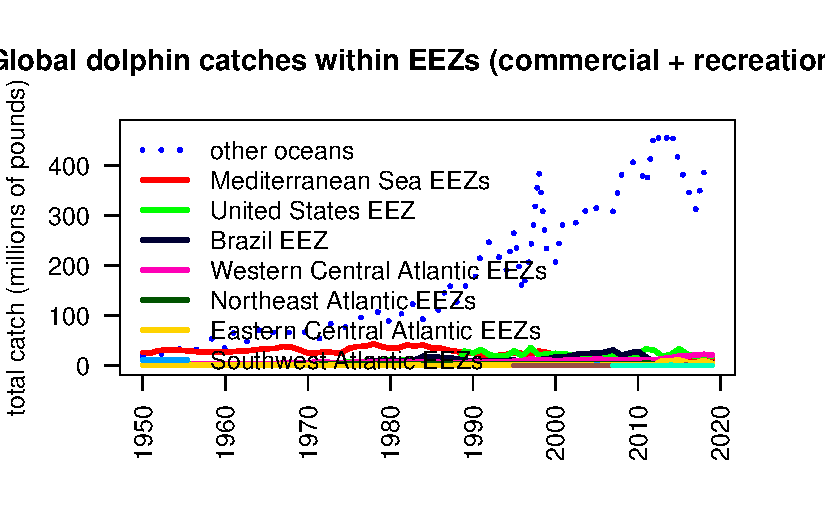
\includegraphics{SAU2_files/figure-pdf/unnamed-chunk-10-1.pdf}

We can see that the EEZ catches globally are dominated by areas outside
of the Atlantic (``other oceans'') so we will replot the data after
moving this category. Here we can see that most of the catches
historically were coming from the Mediterranean Sea, though these
catches have been declining drastially since the 1970s. Catches in the
United States have showed an opposite pattern, with low historical
catches that increased in the 1980s (largely due to the introduction of
recreational monitoring). Catches in the Western Central EEZs have
increased gradually over time.

\begin{Shaded}
\begin{Highlighting}[]
\CommentTok{\# remove other oceans}
\CommentTok{\#head(tab\_glob)}
\NormalTok{tab }\OtherTok{\textless{}{-}}\NormalTok{ tab\_glob[, }\SpecialCharTok{{-}}\FunctionTok{which}\NormalTok{(}\FunctionTok{colnames}\NormalTok{(tab\_glob) }\SpecialCharTok{==} \StringTok{"other oceans"}\NormalTok{)]}
\CommentTok{\#head(tab)}

\FunctionTok{matplot}\NormalTok{(yrs, tab}\SpecialCharTok{/}\DecValTok{10}\SpecialCharTok{\^{}}\DecValTok{6}\NormalTok{, }\AttributeTok{las =} \DecValTok{2}\NormalTok{, }\AttributeTok{type =} \StringTok{"b"}\NormalTok{, }\AttributeTok{pch =} \DecValTok{19}\NormalTok{, }\AttributeTok{cex =} \FloatTok{0.5}\NormalTok{, }\AttributeTok{lty =} \DecValTok{1}\NormalTok{, }\AttributeTok{col =} \FunctionTok{glasbey}\NormalTok{(}\FunctionTok{ncol}\NormalTok{(tab)}\SpecialCharTok{+}\DecValTok{1}\NormalTok{)[}\SpecialCharTok{{-}}\DecValTok{1}\NormalTok{],   }
        \AttributeTok{xlab =} \StringTok{""}\NormalTok{, }\AttributeTok{ylab =} \StringTok{"total catch (millions of pounds)"}\NormalTok{, }\AttributeTok{axes =}\NormalTok{ F,}
        \AttributeTok{main =} \StringTok{"Dolphin catches from the Atlantic EEZs (commercial + recreational)"}\NormalTok{)}
\FunctionTok{matplot}\NormalTok{(yrs, tab}\SpecialCharTok{/}\DecValTok{10}\SpecialCharTok{\^{}}\DecValTok{6}\NormalTok{, }\AttributeTok{las =} \DecValTok{2}\NormalTok{, }\AttributeTok{type =} \StringTok{"l"}\NormalTok{, }\AttributeTok{pch =} \DecValTok{19}\NormalTok{, }\AttributeTok{lty =} \DecValTok{1}\NormalTok{, }\AttributeTok{lwd =} \DecValTok{2}\NormalTok{, }\AttributeTok{add =}\NormalTok{ T, }\AttributeTok{col =} \FunctionTok{glasbey}\NormalTok{(}\FunctionTok{ncol}\NormalTok{(tab)}\SpecialCharTok{+}\DecValTok{1}\NormalTok{)[}\SpecialCharTok{{-}}\DecValTok{1}\NormalTok{])}
\FunctionTok{axis}\NormalTok{(}\DecValTok{1}\NormalTok{, }\AttributeTok{at =}\NormalTok{ yrs[}\FunctionTok{seq}\NormalTok{(}\DecValTok{1}\NormalTok{, }\DecValTok{90}\NormalTok{, }\DecValTok{2}\NormalTok{)], }\AttributeTok{las =} \DecValTok{2}\NormalTok{); }\FunctionTok{axis}\NormalTok{(}\DecValTok{2}\NormalTok{); }\FunctionTok{box}\NormalTok{()}
\FunctionTok{legend}\NormalTok{(}\DecValTok{1952}\NormalTok{, }\DecValTok{25}\NormalTok{, }\FunctionTok{colnames}\NormalTok{(tab), }\AttributeTok{col =} \FunctionTok{glasbey}\NormalTok{(}\FunctionTok{ncol}\NormalTok{(tab)}\SpecialCharTok{+}\DecValTok{1}\NormalTok{)[}\SpecialCharTok{{-}}\DecValTok{1}\NormalTok{], }\AttributeTok{pch =} \DecValTok{19}\NormalTok{, }\AttributeTok{lty =} \DecValTok{1}\NormalTok{, }\AttributeTok{lwd =} \DecValTok{2}\NormalTok{, }\AttributeTok{bty =} \StringTok{"n"}\NormalTok{, }\AttributeTok{cex =} \FloatTok{0.6}\NormalTok{)}
\end{Highlighting}
\end{Shaded}

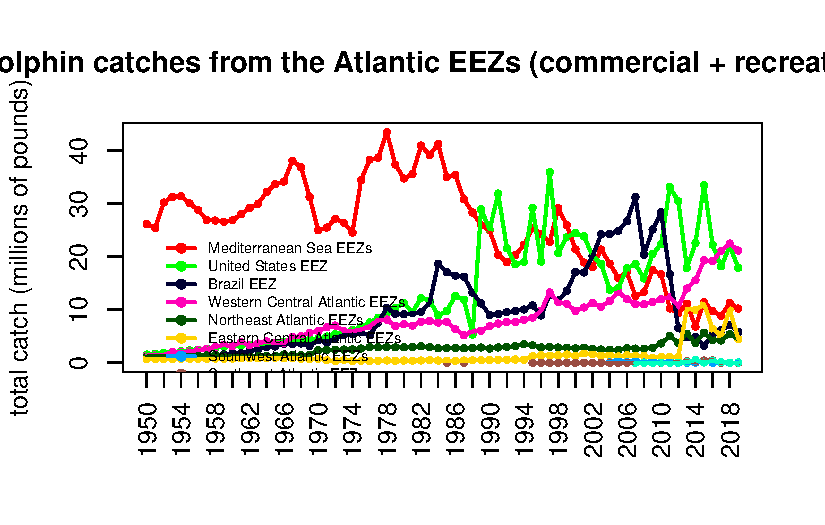
\includegraphics{SAU2_files/figure-pdf/unnamed-chunk-11-1.pdf}

\subsection{Merge high seas with catch with exclusive economic
zones}\label{merge-high-seas-with-catch-with-exclusive-economic-zones}

Now we will merge in the high seas catch from the steps above into the
EEZ catches to get a better picture of total catch in FAO zones 31 and
21. Recall that the U.S. Gulf and Atlantic catches are not necessarily
parsed apart correctly in the public databases which get compiled into
Sea Around Us, so these will have the same deficiencies as noted in
Section 2. Later we will merge in the corrected data.

\begin{Shaded}
\begin{Highlighting}[]
\NormalTok{hs }\OtherTok{\textless{}{-}} \FunctionTok{read.csv}\NormalTok{(}\StringTok{"data/SAU/high\_seas\_by\_year.csv"}\NormalTok{)}
\FunctionTok{names}\NormalTok{(hs)[}\DecValTok{1}\NormalTok{] }\OtherTok{\textless{}{-}} \StringTok{"year"}

\CommentTok{\# check that columns match}
\CommentTok{\#head(tab)}
\CommentTok{\#head(hs)}
\FunctionTok{table}\NormalTok{(}\FunctionTok{rownames}\NormalTok{(tab) }\SpecialCharTok{==}\NormalTok{ hs}\SpecialCharTok{$}\NormalTok{year)  }
\end{Highlighting}
\end{Shaded}

\begin{verbatim}

TRUE 
  70 
\end{verbatim}

\begin{Shaded}
\begin{Highlighting}[]
\NormalTok{tab[}\FunctionTok{which}\NormalTok{(}\FunctionTok{is.na}\NormalTok{(tab))] }\OtherTok{\textless{}{-}} \DecValTok{0}
\NormalTok{tab\_atl }\OtherTok{\textless{}{-}} \FunctionTok{cbind}\NormalTok{(tab, hs[}\DecValTok{2}\SpecialCharTok{:}\DecValTok{3}\NormalTok{])}

\CommentTok{\# check the merge}
\FunctionTok{head}\NormalTok{(tab\_atl)}
\end{Highlighting}
\end{Shaded}

\begin{verbatim}
     Mediterranean Sea EEZs United States EEZ Brazil EEZ
1950               26162262           1548245    1127242
1951               25410830           1721403    1060734
1952               30206350           1871779    1128992
1953               31275619           2024535    1111008
1954               31383840           2177865    1090492
1955               30056210           2309815    1190424
     Western Central Atlantic EEZs Northeast Atlantic EEZs
1950                       1345027                 1173441
1951                       1467925                 1187386
1952                       1510406                 1193045
1953                       2001465                 1141504
1954                       2069754                 1269523
1955                       2130341                 1405543
     Eastern Central Atlantic EEZs Southwest Atlantic EEZs
1950                      677552.5                       0
1951                      693004.4                       0
1952                      708466.7                       0
1953                      723939.4                       0
1954                      739422.5                       0
1955                      754915.9                       0
     Southeast Atlantic EEZs Canadian EEZ Atlantic..Northwest
1950                       0            0                   0
1951                       0            0                   0
1952                       0            0                   0
1953                       0            0                   0
1954                       0            0                   0
1955                       0            0                   0
     Atlantic..Western.Central
1950                         0
1951                         0
1952                         0
1953                         0
1954                         0
1955                         0
\end{verbatim}

\begin{Shaded}
\begin{Highlighting}[]
\CommentTok{\# separate all WCA catches }
\FunctionTok{unique}\NormalTok{(d}\SpecialCharTok{$}\NormalTok{reg)  }\CommentTok{\# use Western Central, U.S. and Canada}
\end{Highlighting}
\end{Shaded}

\begin{verbatim}
 [1] "other oceans"                  "Western Central Atlantic EEZs"
 [3] "Brazil EEZ"                    "Eastern Central Atlantic EEZs"
 [5] "Mediterranean Sea EEZs"        "Northeast Atlantic EEZs"      
 [7] "United States EEZ"             "Southeast Atlantic EEZs"      
 [9] "Southwest Atlantic EEZs"       "Canadian EEZ"                 
\end{verbatim}

\begin{Shaded}
\begin{Highlighting}[]
\NormalTok{dwc }\OtherTok{\textless{}{-}}\NormalTok{ d[}\FunctionTok{which}\NormalTok{(d}\SpecialCharTok{$}\NormalTok{reg }\SpecialCharTok{==} \StringTok{"Western Central Atlantic EEZs"} \SpecialCharTok{|}\NormalTok{ d}\SpecialCharTok{$}\NormalTok{reg }\SpecialCharTok{==} \StringTok{"United States EEZ"} \SpecialCharTok{|}\NormalTok{ d}\SpecialCharTok{$}\NormalTok{reg }\SpecialCharTok{==} \StringTok{"Canadian EEZ"}\NormalTok{),]}

\CommentTok{\#unique(dwc$area\_name[which(dwc$reg == "United States EEZ")])}
\CommentTok{\#unique(dwc$area\_name[which(dwc$reg == "Canadian EEZ")])}
\CommentTok{\#unique(dwc$area\_name[which(dwc$reg == "Western Central Atlantic EEZs")])}

\CommentTok{\# relabel U.S. by area}
\NormalTok{dwc}\SpecialCharTok{$}\NormalTok{reg[}\FunctionTok{which}\NormalTok{(dwc}\SpecialCharTok{$}\NormalTok{area\_name }\SpecialCharTok{==} \StringTok{"USA (East Coast)"}\NormalTok{)] }\OtherTok{\textless{}{-}} \StringTok{"United States East Coast"}
\NormalTok{dwc}\SpecialCharTok{$}\NormalTok{reg[}\FunctionTok{which}\NormalTok{(dwc}\SpecialCharTok{$}\NormalTok{area\_name }\SpecialCharTok{==} \StringTok{"USA (Gulf of Mexico)"}\NormalTok{)] }\OtherTok{\textless{}{-}} \StringTok{"United States Gulf"}
\NormalTok{dwc}\SpecialCharTok{$}\NormalTok{reg[}\FunctionTok{which}\NormalTok{(dwc}\SpecialCharTok{$}\NormalTok{area\_name }\SpecialCharTok{==} \StringTok{"Puerto Rico (USA)"}\NormalTok{)] }\OtherTok{\textless{}{-}} \StringTok{"United States Caribbean"}
\NormalTok{dwc}\SpecialCharTok{$}\NormalTok{reg[}\FunctionTok{which}\NormalTok{(dwc}\SpecialCharTok{$}\NormalTok{area\_name }\SpecialCharTok{==} \StringTok{"US Virgin Isl."}\NormalTok{)] }\OtherTok{\textless{}{-}} \StringTok{"United States Caribbean"}
\CommentTok{\#table(dwc$area\_name, dwc$reg)}

\NormalTok{tab\_wc }\OtherTok{\textless{}{-}} \FunctionTok{tapply}\NormalTok{(dwc}\SpecialCharTok{$}\NormalTok{lbs, }\FunctionTok{list}\NormalTok{(dwc}\SpecialCharTok{$}\NormalTok{year, dwc}\SpecialCharTok{$}\NormalTok{reg), sum, }\AttributeTok{na.rm =}\NormalTok{ T)}
\CommentTok{\#head(tab\_wc)}

\CommentTok{\# reorder S to N}
\NormalTok{tab\_wc }\OtherTok{\textless{}{-}}\NormalTok{ tab\_wc[, }\FunctionTok{c}\NormalTok{(}\DecValTok{5}\NormalTok{, }\DecValTok{2}\NormalTok{, }\DecValTok{4}\NormalTok{, }\DecValTok{3}\NormalTok{, }\DecValTok{1}\NormalTok{)]}
\FunctionTok{head}\NormalTok{(tab\_wc)}
\end{Highlighting}
\end{Shaded}

\begin{verbatim}
     Western Central Atlantic EEZs United States Caribbean United States Gulf
1950                       1202464                142562.8           309225.3
1951                       1299559                168365.6           339921.3
1952                       1341943                168463.5           370512.4
1953                       1839330                162135.2           400578.5
1954                       1901095                168659.3           433479.6
1955                       1954511                175830.1           463752.0
     United States East Coast Canadian EEZ
1950                  1239020           NA
1951                  1381482           NA
1952                  1501267           NA
1953                  1623956           NA
1954                  1744386           NA
1955                  1846063           NA
\end{verbatim}

\begin{Shaded}
\begin{Highlighting}[]
\CommentTok{\# merge in the high seas catch {-} check years match}
\CommentTok{\#head(hs)}
\FunctionTok{table}\NormalTok{(}\FunctionTok{rownames}\NormalTok{(tab\_wc) }\SpecialCharTok{==}\NormalTok{ hs}\SpecialCharTok{$}\NormalTok{year)}
\end{Highlighting}
\end{Shaded}

\begin{verbatim}

TRUE 
  70 
\end{verbatim}

\begin{Shaded}
\begin{Highlighting}[]
\NormalTok{high\_seas }\OtherTok{\textless{}{-}}\NormalTok{ hs}\SpecialCharTok{$}\NormalTok{Atlantic..Western.Central }\SpecialCharTok{+}\NormalTok{ hs}\SpecialCharTok{$}\NormalTok{Atlantic..Northwest}
\NormalTok{high\_seas[high\_seas }\SpecialCharTok{==} \DecValTok{0}\NormalTok{] }\OtherTok{\textless{}{-}} \ConstantTok{NA}
\NormalTok{tab\_wc }\OtherTok{\textless{}{-}} \FunctionTok{cbind}\NormalTok{(tab\_wc, high\_seas)}
\FunctionTok{head}\NormalTok{(tab\_wc)}
\end{Highlighting}
\end{Shaded}

\begin{verbatim}
     Western Central Atlantic EEZs United States Caribbean United States Gulf
1950                       1202464                142562.8           309225.3
1951                       1299559                168365.6           339921.3
1952                       1341943                168463.5           370512.4
1953                       1839330                162135.2           400578.5
1954                       1901095                168659.3           433479.6
1955                       1954511                175830.1           463752.0
     United States East Coast Canadian EEZ high_seas
1950                  1239020           NA        NA
1951                  1381482           NA        NA
1952                  1501267           NA        NA
1953                  1623956           NA        NA
1954                  1744386           NA        NA
1955                  1846063           NA        NA
\end{verbatim}

\subsection{Plot Western Atlantic
catches}\label{plot-western-atlantic-catches}

Now we plot the total Western Atlantic catches -- both within the EEZs
and the high seas -- separating by U.S., Canada, and the Western Central
Atlantic (i.e., the Wider Caribbean). Most of the catch is coming from
the United States and the 40 combined Caribbean jurisdictions which
comprise the Western Central Atlantic.

\begin{Shaded}
\begin{Highlighting}[]
\FunctionTok{par}\NormalTok{(}\AttributeTok{mar =} \FunctionTok{c}\NormalTok{(}\DecValTok{5}\NormalTok{, }\DecValTok{4}\NormalTok{, }\DecValTok{4}\NormalTok{, }\DecValTok{3}\NormalTok{), }\AttributeTok{mgp =} \FunctionTok{c}\NormalTok{(}\DecValTok{3}\NormalTok{, }\DecValTok{1}\NormalTok{, }\DecValTok{0}\NormalTok{))}
\FunctionTok{matplot}\NormalTok{(yrs, tab\_wc}\SpecialCharTok{/}\DecValTok{10}\SpecialCharTok{\^{}}\DecValTok{6}\NormalTok{, }\AttributeTok{las =} \DecValTok{2}\NormalTok{, }\AttributeTok{type =} \StringTok{"l"}\NormalTok{, }\AttributeTok{lty =} \DecValTok{1}\NormalTok{, }\AttributeTok{lwd =} \DecValTok{3}\NormalTok{, }\AttributeTok{col =} \FunctionTok{c}\NormalTok{(}\DecValTok{1}\NormalTok{, }\DecValTok{3}\SpecialCharTok{:}\DecValTok{7}\NormalTok{), }
        \AttributeTok{xlab =} \StringTok{""}\NormalTok{, }\AttributeTok{ylab =} \StringTok{"total catch (millions of pounds)"}\NormalTok{, }
        \AttributeTok{main =} \StringTok{"Western Atlantic dolphin catches (commercial + recreational)"}\NormalTok{)}
\FunctionTok{legend}\NormalTok{(}\StringTok{"topleft"}\NormalTok{, }\FunctionTok{colnames}\NormalTok{(tab\_wc), }\AttributeTok{col =} \FunctionTok{c}\NormalTok{(}\DecValTok{1}\NormalTok{, }\DecValTok{3}\SpecialCharTok{:}\DecValTok{7}\NormalTok{), }\AttributeTok{lty =} \DecValTok{1}\NormalTok{, }\AttributeTok{lwd =} \DecValTok{3}\NormalTok{, }\AttributeTok{bty =} \StringTok{"n"}\NormalTok{)}
\end{Highlighting}
\end{Shaded}

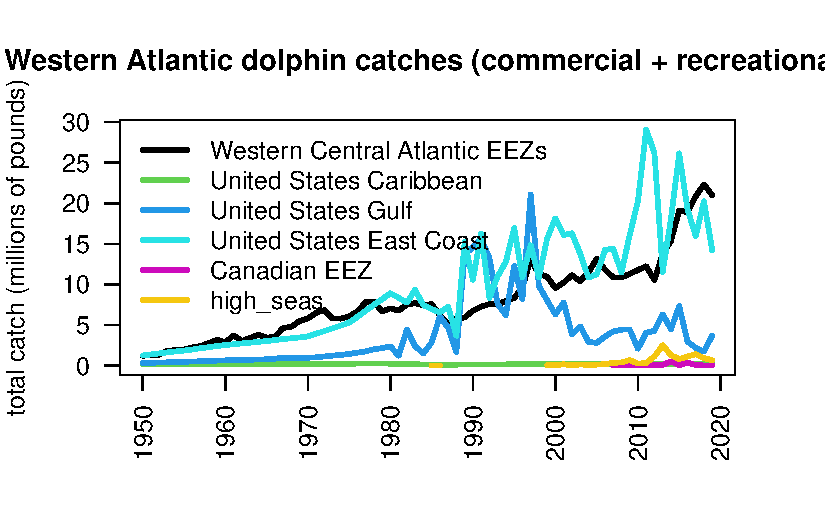
\includegraphics{SAU2_files/figure-pdf/unnamed-chunk-13-1.pdf}

Separating out the mainland United States catches, here are the
international and domestic (mainland) catches plotted over time.

\begin{Shaded}
\begin{Highlighting}[]
\NormalTok{tab\_int }\OtherTok{\textless{}{-}}\NormalTok{ tab\_wc[, }\FunctionTok{c}\NormalTok{(}\DecValTok{1}\NormalTok{, }\DecValTok{2}\NormalTok{, }\DecValTok{5}\NormalTok{, }\DecValTok{6}\NormalTok{)]}
\FunctionTok{head}\NormalTok{(tab\_int)}
\end{Highlighting}
\end{Shaded}

\begin{verbatim}
     Western Central Atlantic EEZs United States Caribbean Canadian EEZ
1950                       1202464                142562.8           NA
1951                       1299559                168365.6           NA
1952                       1341943                168463.5           NA
1953                       1839330                162135.2           NA
1954                       1901095                168659.3           NA
1955                       1954511                175830.1           NA
     high_seas
1950        NA
1951        NA
1952        NA
1953        NA
1954        NA
1955        NA
\end{verbatim}

\begin{Shaded}
\begin{Highlighting}[]
\NormalTok{int\_catch }\OtherTok{\textless{}{-}} \FunctionTok{round}\NormalTok{(}\FunctionTok{rowSums}\NormalTok{(tab\_int, }\AttributeTok{na.rm =}\NormalTok{ T), }\DecValTok{2}\NormalTok{)}
\NormalTok{dom\_catch }\OtherTok{\textless{}{-}} \FunctionTok{rowSums}\NormalTok{(tab\_wc[, }\FunctionTok{c}\NormalTok{(}\DecValTok{3}\NormalTok{, }\DecValTok{4}\NormalTok{)], }\AttributeTok{na.rm =}\NormalTok{ T)}

\FunctionTok{matplot}\NormalTok{(yrs, }\FunctionTok{cbind}\NormalTok{(int\_catch, dom\_catch)}\SpecialCharTok{/}\DecValTok{10}\SpecialCharTok{\^{}}\DecValTok{6}\NormalTok{, }\AttributeTok{las =} \DecValTok{2}\NormalTok{, }\AttributeTok{type =} \StringTok{"l"}\NormalTok{, }\AttributeTok{lty =} \DecValTok{1}\NormalTok{, }\AttributeTok{lwd =} \DecValTok{3}\NormalTok{, }\AttributeTok{col =} \FunctionTok{c}\NormalTok{(}\DecValTok{2}\NormalTok{, }\DecValTok{4}\NormalTok{),}
        \AttributeTok{xlab =} \StringTok{""}\NormalTok{, }\AttributeTok{ylab =} \StringTok{"total catch (millions of pounds)"}\NormalTok{, }
        \AttributeTok{main =} \StringTok{"Western Atlantic dolphin catches in international vs domestic waters}\SpecialCharTok{\textbackslash{}n}\StringTok{(FAO areas 21 and 31, commercial + recreational)"}\NormalTok{)}
\FunctionTok{legend}\NormalTok{(}\StringTok{"topleft"}\NormalTok{, }\FunctionTok{c}\NormalTok{(}\StringTok{"international"}\NormalTok{, }\StringTok{"United States mainland"}\NormalTok{), }\AttributeTok{col =} \FunctionTok{c}\NormalTok{(}\DecValTok{2}\NormalTok{, }\DecValTok{4}\NormalTok{), }\AttributeTok{lty =} \DecValTok{1}\NormalTok{, }\AttributeTok{lwd =} \DecValTok{3}\NormalTok{, }\AttributeTok{bty =} \StringTok{"n"}\NormalTok{)}
\end{Highlighting}
\end{Shaded}

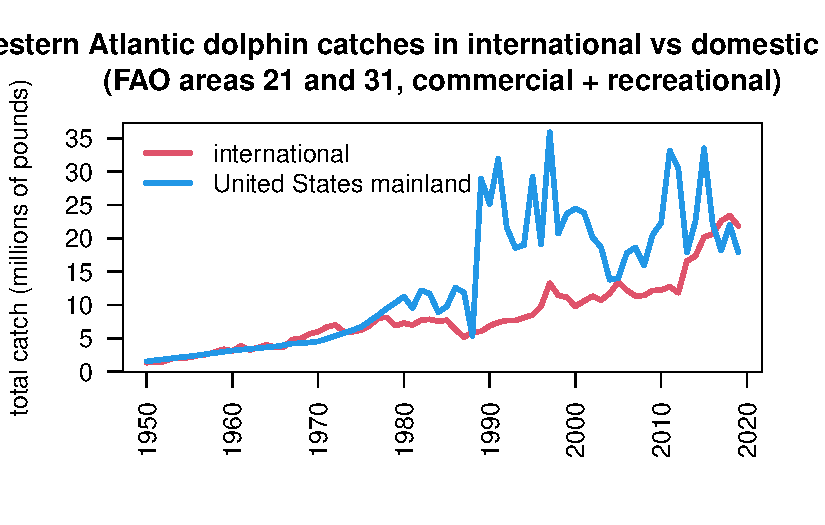
\includegraphics{SAU2_files/figure-pdf/unnamed-chunk-14-1.pdf}

\begin{Shaded}
\begin{Highlighting}[]
\CommentTok{\# output international catches}
\FunctionTok{write.csv}\NormalTok{(}\FunctionTok{data.frame}\NormalTok{(int\_catch), }\AttributeTok{file =} \StringTok{"data/international\_catches.csv"}\NormalTok{, }\AttributeTok{row.names =}\NormalTok{ T)}
\end{Highlighting}
\end{Shaded}

\subsection{Look at Venezuela catches in
detail}\label{look-at-venezuela-catches-in-detail}

Note in the plot above a rapid increase in international catches within
the Western Atlantic. This is driven by a sudden increase in catches
reported within Sea Around Us within the EEZ. We investigate these
catches in detail as it seems odd that a relatively small fleet would be
able to ramp up effort so rapidly. Data can be downloaded on a
country-specific basis, the catches by taxon in the waters of Venezuela
are accessed
\href{https://www.seaaroundus.org/data/\#/eez/862?chart=catch-chart&dimension=taxon&measure=tonnage&limit=10}{here}.

\begin{Shaded}
\begin{Highlighting}[]
\FunctionTok{rm}\NormalTok{(}\AttributeTok{list =} \FunctionTok{ls}\NormalTok{())  }\CommentTok{\# clear the workspace}

\CommentTok{\# download the data for waters of Venezuela}
\NormalTok{ven }\OtherTok{\textless{}{-}} \FunctionTok{read.csv}\NormalTok{(}\StringTok{"data/SAU/SAU EEZ 862 v50{-}1.csv"}\NormalTok{)  }

\CommentTok{\# subset dolphinfish from the data}
\NormalTok{v }\OtherTok{\textless{}{-}}\NormalTok{ ven[}\FunctionTok{which}\NormalTok{(ven}\SpecialCharTok{$}\NormalTok{common\_name }\SpecialCharTok{==} \StringTok{"Common dolphinfish"}\NormalTok{), ]}

\CommentTok{\#apply(v[1:13], 2, table)}

\CommentTok{\#convert to pounds}
\NormalTok{v}\SpecialCharTok{$}\NormalTok{pounds }\OtherTok{\textless{}{-}}\NormalTok{ v}\SpecialCharTok{$}\NormalTok{tonnes }\SpecialCharTok{*} \DecValTok{1000} \SpecialCharTok{*} \FloatTok{2.20462}

\CommentTok{\# look at the characteristics of the data}
\FunctionTok{par}\NormalTok{(}\AttributeTok{mar =} \FunctionTok{c}\NormalTok{(}\DecValTok{5}\NormalTok{, }\DecValTok{10}\NormalTok{, }\DecValTok{1}\NormalTok{, }\DecValTok{1}\NormalTok{), }\AttributeTok{mfrow =} \FunctionTok{c}\NormalTok{(}\DecValTok{3}\NormalTok{, }\DecValTok{2}\NormalTok{), }\AttributeTok{mex =} \FloatTok{0.5}\NormalTok{)}
\CommentTok{\#barplot(tapply(v$pounds/10\^{}6, v$area\_name, sum, na.rm = T), las = 2, xlab = "millions of pounds", main = "Area name", horiz = T)}
\CommentTok{\#barplot(tapply(v$pounds/10\^{}6, v$area\_type, sum, na.rm = T), las = 2, xlab = "millions of pounds", main = "Area type", horiz = T)}
\FunctionTok{barplot}\NormalTok{(}\FunctionTok{tapply}\NormalTok{(v}\SpecialCharTok{$}\NormalTok{pounds}\SpecialCharTok{/}\DecValTok{10}\SpecialCharTok{\^{}}\DecValTok{6}\NormalTok{, v}\SpecialCharTok{$}\NormalTok{year, sum, }\AttributeTok{na.rm =}\NormalTok{ T), }\AttributeTok{las =} \DecValTok{2}\NormalTok{, }\AttributeTok{xlab =} \StringTok{"millions of pounds"}\NormalTok{, }\AttributeTok{main =} \StringTok{"Fishing entity"}\NormalTok{, }\AttributeTok{horiz =}\NormalTok{ T)}
\FunctionTok{barplot}\NormalTok{(}\FunctionTok{tapply}\NormalTok{(v}\SpecialCharTok{$}\NormalTok{pounds}\SpecialCharTok{/}\DecValTok{10}\SpecialCharTok{\^{}}\DecValTok{6}\NormalTok{, v}\SpecialCharTok{$}\NormalTok{fishing\_entity, sum, }\AttributeTok{na.rm =}\NormalTok{ T), }\AttributeTok{las =} \DecValTok{2}\NormalTok{, }\AttributeTok{xlab =} \StringTok{"millions of pounds"}\NormalTok{, }\AttributeTok{main =} \StringTok{"Fishing entity"}\NormalTok{, }\AttributeTok{horiz =}\NormalTok{ T)}
\FunctionTok{barplot}\NormalTok{(}\FunctionTok{tapply}\NormalTok{(v}\SpecialCharTok{$}\NormalTok{pounds}\SpecialCharTok{/}\DecValTok{10}\SpecialCharTok{\^{}}\DecValTok{6}\NormalTok{, v}\SpecialCharTok{$}\NormalTok{fishing\_sector, sum, }\AttributeTok{na.rm =}\NormalTok{ T), }\AttributeTok{las =} \DecValTok{2}\NormalTok{, }\AttributeTok{xlab =} \StringTok{"millions of pounds"}\NormalTok{, }\AttributeTok{main =} \StringTok{"Fishing sector"}\NormalTok{, }\AttributeTok{horiz =}\NormalTok{ T)}
\FunctionTok{barplot}\NormalTok{(}\FunctionTok{tapply}\NormalTok{(v}\SpecialCharTok{$}\NormalTok{pounds}\SpecialCharTok{/}\DecValTok{10}\SpecialCharTok{\^{}}\DecValTok{6}\NormalTok{, v}\SpecialCharTok{$}\NormalTok{catch\_type, sum, }\AttributeTok{na.rm =}\NormalTok{ T), }\AttributeTok{las =} \DecValTok{2}\NormalTok{, }\AttributeTok{xlab =} \StringTok{"millions of pounds"}\NormalTok{, }\AttributeTok{main =} \StringTok{"Catch type"}\NormalTok{, }\AttributeTok{horiz =}\NormalTok{ T)}
\FunctionTok{barplot}\NormalTok{(}\FunctionTok{tapply}\NormalTok{(v}\SpecialCharTok{$}\NormalTok{pounds}\SpecialCharTok{/}\DecValTok{10}\SpecialCharTok{\^{}}\DecValTok{6}\NormalTok{, v}\SpecialCharTok{$}\NormalTok{reporting\_status, sum, }\AttributeTok{na.rm =}\NormalTok{ T), }\AttributeTok{las =} \DecValTok{2}\NormalTok{, }\AttributeTok{xlab =} \StringTok{"millions of pounds"}\NormalTok{, }\AttributeTok{main =} \StringTok{"Reporting status"}\NormalTok{, }\AttributeTok{horiz =}\NormalTok{ T)}
\FunctionTok{barplot}\NormalTok{(}\FunctionTok{tapply}\NormalTok{(v}\SpecialCharTok{$}\NormalTok{pounds}\SpecialCharTok{/}\DecValTok{10}\SpecialCharTok{\^{}}\DecValTok{6}\NormalTok{, v}\SpecialCharTok{$}\NormalTok{gear\_type, sum, }\AttributeTok{na.rm =}\NormalTok{ T), }\AttributeTok{las =} \DecValTok{2}\NormalTok{, }\AttributeTok{xlab =} \StringTok{"millions of pounds"}\NormalTok{, }\AttributeTok{main =} \StringTok{"Gear type"}\NormalTok{, }\AttributeTok{horiz =}\NormalTok{ T)}
\end{Highlighting}
\end{Shaded}

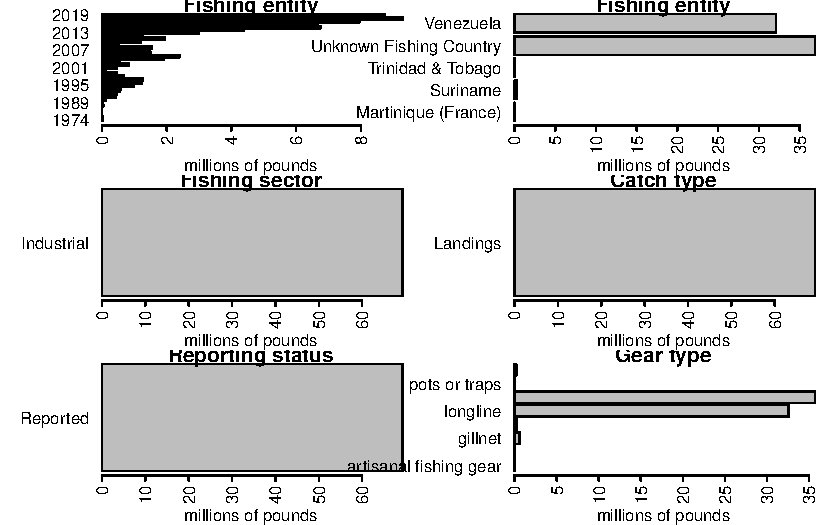
\includegraphics{SAU2_files/figure-pdf/unnamed-chunk-15-1.pdf}

Note that a large portion of the catch in the database is listed as
coming from an ``Unknown Fishing Country.'' We extract these catches and
further investigate the characteristics.

\begin{Shaded}
\begin{Highlighting}[]
\CommentTok{\# extract the Unknown Fishing Country catch}
\NormalTok{v1 }\OtherTok{\textless{}{-}}\NormalTok{ v[}\FunctionTok{which}\NormalTok{(v}\SpecialCharTok{$}\NormalTok{fishing\_entity }\SpecialCharTok{==} \StringTok{"Unknown Fishing Country"}\NormalTok{), ]}
\FunctionTok{apply}\NormalTok{(v1[}\DecValTok{1}\SpecialCharTok{:}\DecValTok{15}\NormalTok{], }\DecValTok{2}\NormalTok{, table)}
\end{Highlighting}
\end{Shaded}

\begin{verbatim}
$area_name

Venezuela 
       39 

$area_type

eez 
 39 

$data_layer

Assigned Tuna RFMO catch 
                      39 

$uncertainty_score
< table of extent 0 >

$year

2013 2014 2015 2016 2017 2018 2019 
   5    5    5    6    7    5    6 

$scientific_name

Coryphaena hippurus 
                 39 

$common_name

Common dolphinfish 
                39 

$functional_group

Large pelagics (>=90 cm) 
                      39 

$commercial_group

Perch-likes 
         39 

$fishing_entity

Unknown Fishing Country 
                     39 

$fishing_sector

Industrial 
        39 

$catch_type

Landings 
      39 

$reporting_status

Reported 
      39 

$gear_type

artisanal fishing gear           bottom trawl                gillnet 
                     1                      5                      7 
            hand lines               longline          pole and line 
                     3                      4                      7 
         pots or traps      unknown by source 
                     5                      7 

$end_use_type

Direct human consumption 
                      39 
\end{verbatim}

\begin{Shaded}
\begin{Highlighting}[]
\CommentTok{\# look at characteristics}
\FunctionTok{par}\NormalTok{(}\AttributeTok{mar =} \FunctionTok{c}\NormalTok{(}\DecValTok{3}\NormalTok{, }\DecValTok{10}\NormalTok{, }\DecValTok{1}\NormalTok{, }\DecValTok{5}\NormalTok{), }\AttributeTok{mfrow =} \FunctionTok{c}\NormalTok{(}\DecValTok{2}\NormalTok{, }\DecValTok{2}\NormalTok{), }\AttributeTok{mex =} \FloatTok{0.6}\NormalTok{)}
\FunctionTok{barplot}\NormalTok{(}\FunctionTok{tapply}\NormalTok{(v1}\SpecialCharTok{$}\NormalTok{pounds}\SpecialCharTok{/}\DecValTok{10}\SpecialCharTok{\^{}}\DecValTok{6}\NormalTok{, v1}\SpecialCharTok{$}\NormalTok{year, sum, }\AttributeTok{na.rm =}\NormalTok{ T), }\AttributeTok{las =} \DecValTok{2}\NormalTok{, }\AttributeTok{xlab =} \StringTok{"millions of pounds"}\NormalTok{, }\AttributeTok{main =} \StringTok{"Year"}\NormalTok{, }\AttributeTok{horiz =}\NormalTok{ T)}
\FunctionTok{barplot}\NormalTok{(}\FunctionTok{tapply}\NormalTok{(v1}\SpecialCharTok{$}\NormalTok{pounds}\SpecialCharTok{/}\DecValTok{10}\SpecialCharTok{\^{}}\DecValTok{6}\NormalTok{, v1}\SpecialCharTok{$}\NormalTok{fishing\_entity, sum, }\AttributeTok{na.rm =}\NormalTok{ T), }\AttributeTok{las =} \DecValTok{2}\NormalTok{, }\AttributeTok{xlab =} \StringTok{"millions of pounds"}\NormalTok{, }\AttributeTok{main =} \StringTok{"Fishing entity"}\NormalTok{, }\AttributeTok{horiz =}\NormalTok{ T)}
\FunctionTok{barplot}\NormalTok{(}\FunctionTok{tapply}\NormalTok{(v1}\SpecialCharTok{$}\NormalTok{pounds}\SpecialCharTok{/}\DecValTok{10}\SpecialCharTok{\^{}}\DecValTok{6}\NormalTok{, v1}\SpecialCharTok{$}\NormalTok{reporting\_status, sum, }\AttributeTok{na.rm =}\NormalTok{ T), }\AttributeTok{las =} \DecValTok{2}\NormalTok{, }\AttributeTok{xlab =} \StringTok{"millions of pounds"}\NormalTok{, }\AttributeTok{main =} \StringTok{"Reporting status"}\NormalTok{, }\AttributeTok{horiz =}\NormalTok{ T)}
\FunctionTok{barplot}\NormalTok{(}\FunctionTok{tapply}\NormalTok{(v1}\SpecialCharTok{$}\NormalTok{pounds}\SpecialCharTok{/}\DecValTok{10}\SpecialCharTok{\^{}}\DecValTok{6}\NormalTok{, v1}\SpecialCharTok{$}\NormalTok{gear\_type, sum, }\AttributeTok{na.rm =}\NormalTok{ T), }\AttributeTok{las =} \DecValTok{2}\NormalTok{, }\AttributeTok{xlab =} \StringTok{"millions of pounds"}\NormalTok{, }\AttributeTok{main =} \StringTok{"Gear type"}\NormalTok{, }\AttributeTok{horiz =}\NormalTok{ T)}
\end{Highlighting}
\end{Shaded}

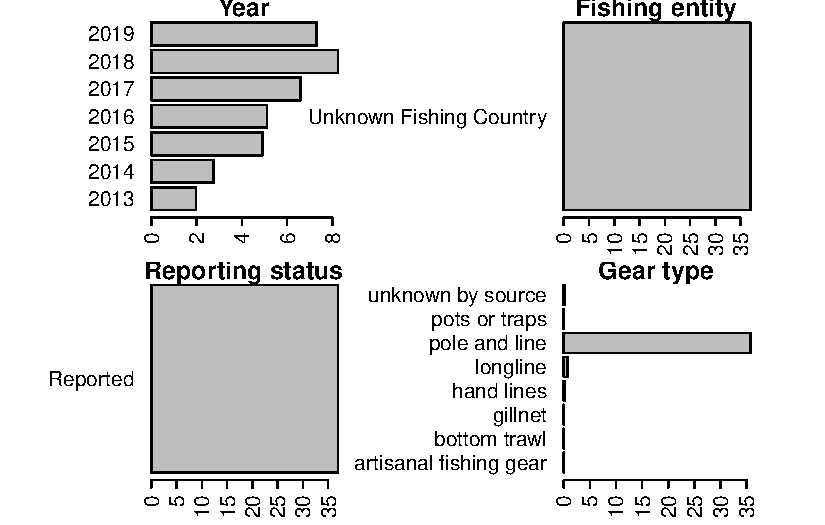
\includegraphics{SAU2_files/figure-pdf/unnamed-chunk-16-1.pdf}

Here is another look at the catches within the venezuelan EEZ, separated
by fishing entity.

\begin{Shaded}
\begin{Highlighting}[]
\CommentTok{\# summarize Venezuela EEZ catches by fishing entity}
\NormalTok{tab }\OtherTok{\textless{}{-}} \FunctionTok{tapply}\NormalTok{(v}\SpecialCharTok{$}\NormalTok{pounds, }\FunctionTok{list}\NormalTok{(v}\SpecialCharTok{$}\NormalTok{year, v}\SpecialCharTok{$}\NormalTok{fishing\_entity), sum, }\AttributeTok{na.rm =}\NormalTok{ T)}
\FunctionTok{head}\NormalTok{(tab)}
\end{Highlighting}
\end{Shaded}

\begin{verbatim}
     Martinique (France) Suriname Trinidad & Tobago Unknown Fishing Country
1974            7320.429       NA                NA                      NA
1976           12814.641       NA                NA                      NA
1985                  NA       NA                NA                      NA
1986                  NA       NA                NA                      NA
1987                  NA       NA                NA                      NA
1988                  NA       NA                NA                      NA
     Venezuela
1974        NA
1976        NA
1985  4699.563
1986  2229.484
1987  4585.610
1988 39960.149
\end{verbatim}

\begin{Shaded}
\begin{Highlighting}[]
\FunctionTok{matplot}\NormalTok{(}\FunctionTok{rownames}\NormalTok{(tab), tab}\SpecialCharTok{/}\DecValTok{10}\SpecialCharTok{\^{}}\DecValTok{6}\NormalTok{, }\AttributeTok{las =} \DecValTok{2}\NormalTok{, }\AttributeTok{type =} \StringTok{"b"}\NormalTok{, }\AttributeTok{lty =} \DecValTok{1}\NormalTok{, }\AttributeTok{lwd =} \DecValTok{2}\NormalTok{, }\AttributeTok{pch =} \DecValTok{19}\NormalTok{, }\AttributeTok{col =} \DecValTok{1}\SpecialCharTok{:}\DecValTok{5}\NormalTok{,}
        \AttributeTok{xlab =} \StringTok{""}\NormalTok{, }\AttributeTok{ylab =} \StringTok{"total catch (millions of pounds)"}\NormalTok{, }\AttributeTok{axes =}\NormalTok{ F, }
        \AttributeTok{main =} \StringTok{"Total dolphinfish catches in the Venezuelan EEZ"}\NormalTok{)}
\FunctionTok{axis}\NormalTok{(}\DecValTok{1}\NormalTok{, }\AttributeTok{at =} \FunctionTok{seq}\NormalTok{(}\DecValTok{1950}\NormalTok{, }\DecValTok{2020}\NormalTok{, }\DecValTok{5}\NormalTok{)); }\FunctionTok{axis}\NormalTok{(}\DecValTok{2}\NormalTok{, }\AttributeTok{las =} \DecValTok{2}\NormalTok{); }\FunctionTok{box}\NormalTok{()}
\FunctionTok{legend}\NormalTok{(}\StringTok{"topleft"}\NormalTok{, }\FunctionTok{colnames}\NormalTok{(tab), }\AttributeTok{col =} \DecValTok{1}\SpecialCharTok{:}\DecValTok{5}\NormalTok{, }\AttributeTok{pch =} \DecValTok{19}\NormalTok{, }\AttributeTok{lty =} \DecValTok{1}\NormalTok{, }\AttributeTok{lwd =} \DecValTok{3}\NormalTok{, }\AttributeTok{bty =} \StringTok{"n"}\NormalTok{, }\AttributeTok{title =} \StringTok{"Fishing entity"}\NormalTok{)}

\FunctionTok{text}\NormalTok{(}\DecValTok{2004}\NormalTok{, }\DecValTok{6}\NormalTok{, }\AttributeTok{cex =} \FloatTok{0.8}\NormalTok{,}
     \StringTok{"These Unknown Fishing Country}\SpecialCharTok{\textbackslash{}n}\StringTok{catches appear in the database as an}\SpecialCharTok{\textbackslash{}n}\StringTok{industrial fleet using pole and line gear}\SpecialCharTok{\textbackslash{}n}\StringTok{and are all listed as reported data}\SpecialCharTok{\textbackslash{}n}\StringTok{(\textquotesingle{}Assigned Tuna RFMO catch\textquotesingle{})"}\NormalTok{)}
\end{Highlighting}
\end{Shaded}

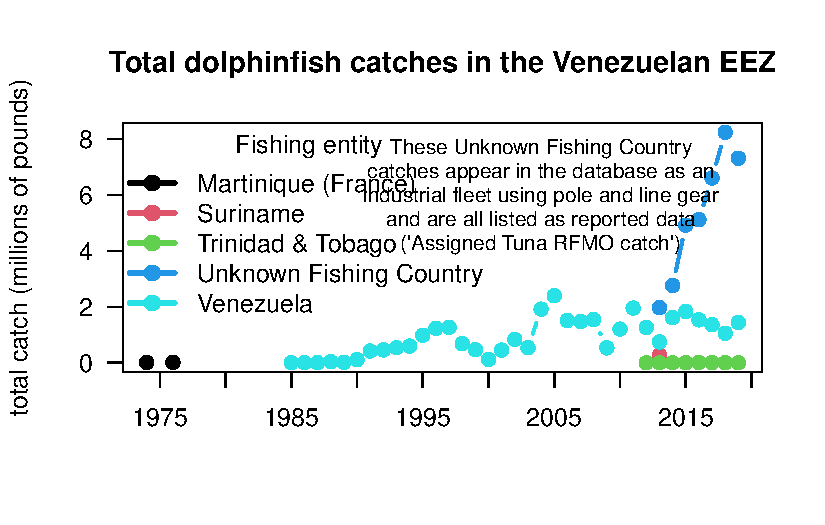
\includegraphics{SAU2_files/figure-pdf/unnamed-chunk-17-1.pdf}

The very substantial increase in international Western Atlantic dolphin
catches can be attributed solely to this Unknown Fishing Country catches
which appear in the database beginning in 2013. The documentation of the
catch reconstruction can be found in the Sea Around Us documentation
files (see Mendoza et al.~2015). We spoke to Jeremy Mendoza and other
experts who were involved in the reconstruction of domestic catches in
Venezuela, and they noted that the ``Assigned tuna RFMO catch'' actually
emerge from spatially reshuffled landing reports to ICCAT, according to
the methods of
\href{https://www.sciencedirect.com/science/article/abs/pii/S0165783619302346}{Coulter
et al.~(2020)}. In this work, the Sea Around Us team developed a global
spatial reallocation of landings of tunas and associated species that
were reported to ICCAT. In short, this work uses the fraction of
reported spatially disaggregated data to reallocate all data reported to
ICCAT. This step is necessary because there are not many countries that
report spatial data to ICCAT in the region, and this method may lead to
a significant reallocation of landings from the Caribbean to the
Venezuelan EEZ, where the local pole and line fishery is significant (J.
Mendoza, personal communication). Thus, it is likely that landings from
other EEZs, that were included in the reconstructed catch data layer,
could have been reassigned to the Venezuelan EEZ.

Because there may be some overlap between the reconstructed data used in
the national EEZ estimates, and the ICCAT reporting that was reassigned,
there could potentially be a ``double counting'' of these catch
estimates in the Sea Around Us database. These Unknown Fishing Country
catches that lead to a large increase in total estimated catches within
the Venezuelan EEZ should be treated with caution at this time, until we
can verify with Sea Around Us database managers that the spatial
disaggregation method used has not led to an overestimate.

\subsection{Distribute the high seas landings across quarters of the
year}\label{distribute-the-high-seas-landings-across-quarters-of-the-year-1}

The international landings are only reported as annual catches and do
not have any month or season associated with them. However, the MSE
operating model requires seasonal catches. The majority of the
international landings are caught by longline, so we will assume that
the fleet distribution of the U.S. pelagic longline is representative of
the seasonality of the international high seas fleets. Now we parse the
annual catches according to the seasonality of the U.S. fleet.

At the time of analysis, the SAU database only contained catches to
2019, so we interpolated the 2019 values to cover years 2020 - 2022.

\begin{Shaded}
\begin{Highlighting}[]
\CommentTok{\# read in the percentage of the catch by area and year{-}quarter combinations from the U.S. PLL}
\FunctionTok{load}\NormalTok{(}\StringTok{"data/per\_PLLcatch\_by\_area\_yearquarter.RData"}\NormalTok{)  }

\NormalTok{percatch[, , }\DecValTok{7}\NormalTok{] }\CommentTok{\# these are the percentages for the NED (Atlantic Northwest)}
\end{Highlighting}
\end{Shaded}

\begin{verbatim}
        1997       1998      1999        2000      2001       2002      2003
1 0.00000000 0.00000000 0.0000000 0.000000000 0.0000000 0.02866242 0.0000000
2 0.72895277 0.00000000 0.0000000 0.173761946 0.0000000 0.35668790 0.0000000
3 0.23425736 0.97257268 0.8203593 0.816681147 0.7959184 0.56050955 0.2345836
4 0.03678987 0.02742732 0.1796407 0.009556907 0.2040816 0.05414013 0.7654164
  2004 2005 2006       2007       2008        2009      2010 2011       2012
1    0  0.0    0 0.00000000 0.00000000 0.000000000 0.0000000    0 0.00000000
2    0  0.0    0 0.09846154 0.04568528 0.720183486 0.0000000    0 0.02208202
3    1  0.5    1 0.90153846 0.77157360 0.270642202 0.4885057    1 0.92744479
4    0  0.5    0 0.00000000 0.18274112 0.009174312 0.5114943    0 0.05047319
        2013      2014      2015      2016       2017       2018 2019 2020 2021
1 0.00000000 0.0000000 0.0000000 0.0000000 0.00000000 0.00000000    0    0    0
2 0.08898776 0.0000000 0.0000000 0.0000000 0.00000000 0.00000000    0    0    0
3 0.86095662 0.5979299 0.3076923 0.7073171 0.93650794 0.93650794    1    1    1
4 0.05005562 0.4020701 0.6923077 0.2926829 0.06349206 0.06349206    0    0    0
  2022
1    0
2    1
3    0
4    0
\end{verbatim}

\begin{Shaded}
\begin{Highlighting}[]
\NormalTok{tab }\OtherTok{\textless{}{-}}\NormalTok{ tab[}\FunctionTok{which}\NormalTok{(}\FunctionTok{rownames}\NormalTok{(tab) }\SpecialCharTok{\textgreater{}=} \DecValTok{1997}\NormalTok{), ]  }\CommentTok{\# PLL data are only available from 1997 on }
\CommentTok{\#tab[nrow(tab), ]}
\NormalTok{tab }\OtherTok{\textless{}{-}} \FunctionTok{rbind}\NormalTok{(tab, tab[}\FunctionTok{nrow}\NormalTok{(tab), ], tab[}\FunctionTok{nrow}\NormalTok{(tab), ], tab[}\FunctionTok{nrow}\NormalTok{(tab), ])  }\CommentTok{\# interpolate 2019 catches for 2020{-}2022}

\NormalTok{NED }\OtherTok{\textless{}{-}}\NormalTok{ percatch[, , }\DecValTok{1}\NormalTok{]   }\CommentTok{\# create matrices for final catch data}
\NormalTok{NCA }\OtherTok{\textless{}{-}}\NormalTok{ percatch[, , }\DecValTok{1}\NormalTok{]}

\ControlFlowTok{for}\NormalTok{ (i }\ControlFlowTok{in} \DecValTok{1}\SpecialCharTok{:}\FunctionTok{ncol}\NormalTok{(percatch))  \{ }
\NormalTok{  NED[, i] }\OtherTok{\textless{}{-}}\NormalTok{ percatch[, i, }\DecValTok{7}\NormalTok{] }\SpecialCharTok{*}\NormalTok{ tab[i, }\DecValTok{1}\NormalTok{]}
\NormalTok{  NCA[, i] }\OtherTok{\textless{}{-}}\NormalTok{ percatch[, i, }\DecValTok{1}\NormalTok{] }\SpecialCharTok{*}\NormalTok{ tab[i, }\DecValTok{2}\NormalTok{]}
\NormalTok{  \}}

\CommentTok{\# format for operating model}
\NormalTok{yrs }\OtherTok{\textless{}{-}} \FunctionTok{sort}\NormalTok{(}\FunctionTok{rep}\NormalTok{(}\FunctionTok{as.numeric}\NormalTok{(}\FunctionTok{colnames}\NormalTok{(NCA)), }\DecValTok{4}\NormalTok{))}
\NormalTok{qrt }\OtherTok{\textless{}{-}} \FunctionTok{rep}\NormalTok{(}\DecValTok{1}\SpecialCharTok{:}\DecValTok{4}\NormalTok{, }\FunctionTok{length}\NormalTok{(yrs)}\SpecialCharTok{/}\DecValTok{4}\NormalTok{)}
\NormalTok{flt }\OtherTok{\textless{}{-}} \FunctionTok{rep}\NormalTok{(}\StringTok{"Intl"}\NormalTok{, }\FunctionTok{length}\NormalTok{(yrs))}
\NormalTok{are }\OtherTok{\textless{}{-}} \FunctionTok{rep}\NormalTok{(}\StringTok{"NED"}\NormalTok{, }\FunctionTok{length}\NormalTok{(yrs))}
\NormalTok{fin1 }\OtherTok{\textless{}{-}} \FunctionTok{data.frame}\NormalTok{(}\FunctionTok{cbind}\NormalTok{(yrs, qrt, flt, are, }\FunctionTok{matrix}\NormalTok{(NED)))}
\NormalTok{are }\OtherTok{\textless{}{-}} \FunctionTok{rep}\NormalTok{(}\StringTok{"NCA"}\NormalTok{, }\FunctionTok{length}\NormalTok{(yrs))}
\NormalTok{fin2 }\OtherTok{\textless{}{-}} \FunctionTok{data.frame}\NormalTok{(}\FunctionTok{cbind}\NormalTok{(yrs, qrt, flt, are, }\FunctionTok{matrix}\NormalTok{(NCA)))}

\NormalTok{findat }\OtherTok{\textless{}{-}} \FunctionTok{data.frame}\NormalTok{(}\FunctionTok{rbind}\NormalTok{(fin1, fin2), }\AttributeTok{stringsAsFactors =} \ConstantTok{FALSE}\NormalTok{)}
\FunctionTok{names}\NormalTok{(findat) }\OtherTok{\textless{}{-}} \FunctionTok{c}\NormalTok{(}\StringTok{"Year"}\NormalTok{, }\StringTok{"Quarter"}\NormalTok{, }\StringTok{"Fleet"}\NormalTok{, }\StringTok{"Area"}\NormalTok{, }\StringTok{"Catch\_lbs"}\NormalTok{)}
\NormalTok{findat}\SpecialCharTok{$}\NormalTok{Catch\_lbs }\OtherTok{\textless{}{-}} \FunctionTok{as.numeric}\NormalTok{(findat}\SpecialCharTok{$}\NormalTok{Catch\_lbs)}
\FunctionTok{head}\NormalTok{(findat)}
\end{Highlighting}
\end{Shaded}

\begin{verbatim}
  Year Quarter Fleet Area Catch_lbs
1 1997       1  Intl  NED        NA
2 1997       2  Intl  NED        NA
3 1997       3  Intl  NED        NA
4 1997       4  Intl  NED        NA
5 1998       1  Intl  NED        NA
6 1998       2  Intl  NED        NA
\end{verbatim}

\begin{Shaded}
\begin{Highlighting}[]
\CommentTok{\#plot(findat$Catch\_lbs, type = "l")}
\CommentTok{\#plot(findat$Catch\_lbs \textasciitilde{} factor(findat$Area))}
\CommentTok{\#plot(findat$Catch\_lbs \textasciitilde{} factor(findat$Quarter))}
\CommentTok{\#plot(findat$Catch\_lbs \textasciitilde{} factor(findat$Year))}
\CommentTok{\#apply(findat, 2, table)}

\FunctionTok{write.csv}\NormalTok{(findat, }\AttributeTok{file =} \StringTok{"data/outputs/Intl\_highseas\_TomFormat.csv"}\NormalTok{)}

\NormalTok{tab }\OtherTok{\textless{}{-}} \FunctionTok{tapply}\NormalTok{(findat}\SpecialCharTok{$}\NormalTok{Catch\_lbs, }\FunctionTok{list}\NormalTok{(findat}\SpecialCharTok{$}\NormalTok{Quarter, findat}\SpecialCharTok{$}\NormalTok{Area), sum, }\AttributeTok{na.rm =}\NormalTok{ T)}
\CommentTok{\#barplot(tab, beside = T, col = rainbow(4))}

\FunctionTok{matplot}\NormalTok{(yrs }\SpecialCharTok{+}\NormalTok{ qrt}\SpecialCharTok{/}\DecValTok{4}\NormalTok{, }\FunctionTok{cbind}\NormalTok{(}\FunctionTok{as.numeric}\NormalTok{(fin1}\SpecialCharTok{$}\NormalTok{V5), }\FunctionTok{as.numeric}\NormalTok{(fin2}\SpecialCharTok{$}\NormalTok{V5))}\SpecialCharTok{/}\DecValTok{10}\SpecialCharTok{\^{}}\DecValTok{6}\NormalTok{, }\AttributeTok{lty =} \DecValTok{1}\NormalTok{, }\AttributeTok{lwd =} \DecValTok{2}\NormalTok{, }
        \AttributeTok{col =} \DecValTok{2}\SpecialCharTok{:}\DecValTok{3}\NormalTok{, }\AttributeTok{type =} \StringTok{"l"}\NormalTok{, }\AttributeTok{main =} \StringTok{"International high seas catches by quarter"}\NormalTok{, }
        \AttributeTok{xlab =} \StringTok{""}\NormalTok{, }\AttributeTok{ylab =} \StringTok{"total catch (millions of pounds)"}\NormalTok{)}
\FunctionTok{legend}\NormalTok{(}\StringTok{"topleft"}\NormalTok{, }\FunctionTok{c}\NormalTok{(}\StringTok{"NED"}\NormalTok{, }\StringTok{"NCA"}\NormalTok{), }\AttributeTok{lwd =} \DecValTok{2}\NormalTok{, }\AttributeTok{col =} \DecValTok{2}\SpecialCharTok{:}\DecValTok{3}\NormalTok{, }\AttributeTok{bty =} \StringTok{"n"}\NormalTok{)}
\end{Highlighting}
\end{Shaded}

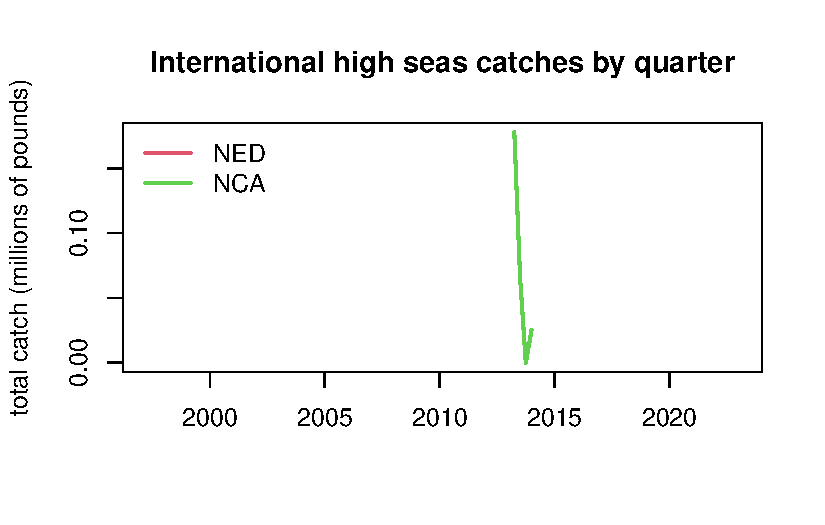
\includegraphics{SAU2_files/figure-pdf/unnamed-chunk-18-1.pdf}

\subsection{References}\label{references}

Pauly D., Zeller D., Palomares M.L.D. (Editors), 2020. Sea Around Us
Concepts, Design and Data (seaaroundus.org).




\end{document}
